% Options for packages loaded elsewhere
\PassOptionsToPackage{unicode}{hyperref}
\PassOptionsToPackage{hyphens}{url}
\PassOptionsToPackage{dvipsnames,svgnames,x11names}{xcolor}
%
\documentclass[
]{article}
\usepackage{amsmath,amssymb}
\usepackage{iftex}
\ifPDFTeX
  \usepackage[T1]{fontenc}
  \usepackage[utf8]{inputenc}
  \usepackage{textcomp} % provide euro and other symbols
\else % if luatex or xetex
  \usepackage{unicode-math} % this also loads fontspec
  \defaultfontfeatures{Scale=MatchLowercase}
  \defaultfontfeatures[\rmfamily]{Ligatures=TeX,Scale=1}
\fi
\usepackage{lmodern}
\ifPDFTeX\else
  % xetex/luatex font selection
\fi
% Use upquote if available, for straight quotes in verbatim environments
\IfFileExists{upquote.sty}{\usepackage{upquote}}{}
\IfFileExists{microtype.sty}{% use microtype if available
  \usepackage[]{microtype}
  \UseMicrotypeSet[protrusion]{basicmath} % disable protrusion for tt fonts
}{}
\makeatletter
\@ifundefined{KOMAClassName}{% if non-KOMA class
  \IfFileExists{parskip.sty}{%
    \usepackage{parskip}
  }{% else
    \setlength{\parindent}{0pt}
    \setlength{\parskip}{6pt plus 2pt minus 1pt}}
}{% if KOMA class
  \KOMAoptions{parskip=half}}
\makeatother
\usepackage{xcolor}
\usepackage[margin=1in]{geometry}
\usepackage{longtable,booktabs,array}
\usepackage{calc} % for calculating minipage widths
% Correct order of tables after \paragraph or \subparagraph
\usepackage{etoolbox}
\makeatletter
\patchcmd\longtable{\par}{\if@noskipsec\mbox{}\fi\par}{}{}
\makeatother
% Allow footnotes in longtable head/foot
\IfFileExists{footnotehyper.sty}{\usepackage{footnotehyper}}{\usepackage{footnote}}
\makesavenoteenv{longtable}
\usepackage{graphicx}
\makeatletter
\def\maxwidth{\ifdim\Gin@nat@width>\linewidth\linewidth\else\Gin@nat@width\fi}
\def\maxheight{\ifdim\Gin@nat@height>\textheight\textheight\else\Gin@nat@height\fi}
\makeatother
% Scale images if necessary, so that they will not overflow the page
% margins by default, and it is still possible to overwrite the defaults
% using explicit options in \includegraphics[width, height, ...]{}
\setkeys{Gin}{width=\maxwidth,height=\maxheight,keepaspectratio}
% Set default figure placement to htbp
\makeatletter
\def\fps@figure{htbp}
\makeatother
\setlength{\emergencystretch}{3em} % prevent overfull lines
\providecommand{\tightlist}{%
  \setlength{\itemsep}{0pt}\setlength{\parskip}{0pt}}
\setcounter{secnumdepth}{5}
\newlength{\cslhangindent}
\setlength{\cslhangindent}{1.5em}
\newlength{\csllabelwidth}
\setlength{\csllabelwidth}{3em}
\newlength{\cslentryspacingunit} % times entry-spacing
\setlength{\cslentryspacingunit}{\parskip}
\newenvironment{CSLReferences}[2] % #1 hanging-ident, #2 entry spacing
 {% don't indent paragraphs
  \setlength{\parindent}{0pt}
  % turn on hanging indent if param 1 is 1
  \ifodd #1
  \let\oldpar\par
  \def\par{\hangindent=\cslhangindent\oldpar}
  \fi
  % set entry spacing
  \setlength{\parskip}{#2\cslentryspacingunit}
 }%
 {}
\usepackage{calc}
\newcommand{\CSLBlock}[1]{#1\hfill\break}
\newcommand{\CSLLeftMargin}[1]{\parbox[t]{\csllabelwidth}{#1}}
\newcommand{\CSLRightInline}[1]{\parbox[t]{\linewidth - \csllabelwidth}{#1}\break}
\newcommand{\CSLIndent}[1]{\hspace{\cslhangindent}#1}
\usepackage{ragged2e}
\usepackage{setspace}
\usepackage{tocloft}
\usepackage{float}
\floatplacement{figure}{H}
\usepackage{wrapfig}
\usepackage{pdfpages}
\usepackage{caption}
\usepackage{booktabs}
\usepackage{longtable}
\usepackage{array}
\usepackage{multirow}
\usepackage{wrapfig}
\usepackage{float}
\usepackage{colortbl}
\usepackage{pdflscape}
\usepackage{tabu}
\usepackage{threeparttable}
\usepackage{threeparttablex}
\usepackage[normalem]{ulem}
\usepackage{makecell}
\usepackage{xcolor}
\ifLuaTeX
  \usepackage{selnolig}  % disable illegal ligatures
\fi
\IfFileExists{bookmark.sty}{\usepackage{bookmark}}{\usepackage{hyperref}}
\IfFileExists{xurl.sty}{\usepackage{xurl}}{} % add URL line breaks if available
\urlstyle{same}
\hypersetup{
  colorlinks=true,
  linkcolor={black},
  filecolor={Maroon},
  citecolor={Blue},
  urlcolor={Blue},
  pdfcreator={LaTeX via pandoc}}

\author{}
\date{\vspace{-2.5em}}

\begin{document}

\thispagestyle{empty}
\begin{singlespace} 
\begin{center}

\Huge

\textbf{HERE GOES YOUR TITLE}

\Large

\vspace{8mm}

by

\vspace{8mm}

\huge

Here Goes Your Name

\Large

\vspace{8mm}

Undergraduate degree

Master degree

\vspace{10mm}

A DISSERTATION SUBMITTED IN PARTIAL FULFILLMENT OF THE REQUIREMENTS FOR THE DEGREE OF

\vspace{5mm}

HERE GOES YOUR DEGREEE

\vspace{5mm}
in

\vspace{5mm}

THE FACULTY OF GRADUATE AND POSTDOCTORAL STUDIES

\vspace{5mm}

(Program)

\vspace{5mm}

THE UNIVERSITY OF BRITISH COLUMBIA

\vspace{5mm}

(Vancouver)

\vspace{6mm}

Month YYYY

© Here Goes Your Name, YYYY

\end{center}
\end{singlespace}
\normalsize
\clearpage

\pagenumbering{roman}
\setcounter{page}{2}

\doublespacing

The following individuals certify that they have read, and recommend to the Faculty of Graduate
and Postdoctoral Studies for acceptance, the dissertation entitled:

\vspace{5mm}

\noindent\underline{\makebox[6in][l]{Insert your dissertation title here}}\\
\vspace{2mm}

submitted by \underline{Insert Your Name Here} in partial fulfillment of the requirements for

the degree of \noindent\underline{\makebox[5in][l]{Name of your Degree}}

in \noindent\underline{\makebox[5.8in][l]{Insert Program}}

\vspace{5mm}

\textbf{Examining Committee:}

\noindent\underline{\makebox[6in][l]{Name of your Supervisor}}\\
Supervisor

\noindent\underline{\makebox[6in][l]{Name of your Committee Member}}\\
Supervisory Committee Member

\noindent\underline{\makebox[6in][l]{Name of University Examiner}}\\
University Examiner

\noindent\underline{\makebox[6in][l]{Name of University Examiner}}\\
University Examiner

\noindent\underline{\makebox[6in][l]{Name of External Examiner}}\\
External Examiner

\textbf{Additional Supervisory Committee Members:}

\noindent\underline{\makebox[6in][l]{Name of your Committee Member}}\\
Supervisory Committee Member

\clearpage

\setlength{\parindent}{4em} 
\linespread{1}
\doublespacing

\section*{Abstract}
\addcontentsline{toc}{section}{Abstract}

Lorem ipsum dolor sit amet, consectetur adipiscing elit. Nulla eleifend odio odio, et consectetur nunc commodo vitae. Donec eu finibus lacus. Integer at porta nulla. Fusce dignissim gravida lacinia. Nulla ut odio in ante imperdiet placerat. Maecenas vel imperdiet lorem. Proin ultricies, ex at bibendum fringilla, neque libero malesuada sem, in tincidunt leo mi vel mi. Phasellus scelerisque sagittis urna sed sodales. Curabitur iaculis justo velit, ultricies euismod justo convallis non. Nunc id purus et ante iaculis dignissim vel non erat. Donec dignissim urna ut lobortis congue. Nulla tempus ut ipsum non ornare. Donec ac purus nec sem cursus eleifend. Suspendisse potenti. Vestibulum ac vehicula ante.

Donec pulvinar a est ut vulputate. In id euismod nisi. Curabitur pulvinar bibendum convallis. Phasellus luctus posuere quam, a dapibus massa tristique in. Sed fermentum fermentum velit non sodales. Donec eget efficitur turpis. Sed ligula diam, ultrices porta vestibulum sed, varius maximus erat. Sed sagittis ut nisi ac tincidunt. Aliquam augue elit, egestas eu commodo ut, eleifend et nulla. Phasellus mollis lacus ac tortor fringilla, eget viverra enim sagittis. Morbi facilisis porttitor dui, eget elementum tellus malesuada ac. Integer sed accumsan lorem. Cras placerat ultrices libero at efficitur. Orci varius natoque penatibus et magnis dis parturient montes, nascetur ridiculus mus.

Nullam magna elit, sodales eu massa a, rutrum gravida orci. Mauris cursus odio turpis, et dignissim neque rutrum sit amet. Mauris vel nibh enim. Vestibulum tempus et lectus quis tempor. Proin dictum dui luctus felis sodales porttitor. Maecenas viverra vestibulum tristique. Nulla facilisi. Quisque efficitur lacus diam. Phasellus eget ligula quis mauris fermentum feugiat. Duis vitae lectus porttitor, vestibulum velit a, tincidunt nulla. Donec pharetra erat et urna sollicitudin, ac iaculis quam pulvinar. Donec pulvinar justo maximus lacinia sodales. Etiam sit amet diam vel ligula tempor congue nec in libero. Donec arcu risus, posuere.

\clearpage

\section*{Lay Summary}
\addcontentsline{toc}{section}{Lay Summary}

Lorem ipsum dolor sit amet, consectetur adipiscing elit. Sed lorem massa, suscipit vel dapibus a, iaculis ut sapien. Duis eu tellus vitae ligula semper commodo. Morbi felis tortor, ullamcorper vitae venenatis sit amet, commodo eu tortor. Proin ultrices ipsum ipsum, sed viverra arcu maximus eget. Aliquam nec nisl rutrum quam tempus iaculis nec sed dui. Nulla vitae imperdiet neque. Morbi eget eleifend lectus. Etiam semper id purus et scelerisque. Suspendisse lectus libero, iaculis et arcu vel, mattis mollis odio.

Phasellus quis metus erat. Nunc erat mi, posuere eleifend tortor quis, consequat dignissim metus. Pellentesque eget ante massa. Integer ultrices pulvinar varius. Sed dapibus sed arcu sit amet cursus. In hac habitasse platea dictumst. Aliquam vehicula est sed velit dapibus commodo. Donec placerat eu metus vel efficitur. Pellentesque commodo, nisi at elementum sagittis, erat magna feugiat elit, sit amet facilisis est diam eget tellus. Ut tellus velit, fringilla non consequat ut.

\clearpage

\section*{Preface}
\addcontentsline{toc}{section}{Preface}

Lorem ipsum dolor sit amet, consectetur adipiscing elit. Cras id nulla malesuada, auctor arcu at, tempor nibh. Etiam ultricies dictum nisi eu vulputate. Suspendisse tempor aliquam efficitur. Curabitur eget orci ac purus hendrerit laoreet. Proin porta arcu nisl, a fermentum tellus suscipit et. Nulla mattis orci ac tortor facilisis venenatis. Phasellus a velit tristique, tincidunt purus id, aliquet tellus. Orci varius natoque penatibus et magnis dis parturient montes, nascetur ridiculus mus. Sed et turpis sed odio faucibus aliquam nec eget est.

Phasellus ligula lacus, euismod posuere pretium sit amet, ornare condimentum nisl. Integer eu aliquet lectus, sit amet sagittis turpis. Etiam tempus bibendum nibh, eu accumsan sapien. Suspendisse tincidunt sit amet nisi vel consectetur. Donec vitae odio elit. Quisque dignissim risus feugiat nunc tempor hendrerit. Fusce consequat lectus eget felis tempus, et lobortis ante ornare. Etiam euismod quam eu scelerisque mattis. Praesent nisi lectus, tincidunt nec sapien ac, fermentum pellentesque orci.

Praesent semper faucibus mauris, in suscipit quam mattis et. Curabitur malesuada placerat magna. Morbi eget bibendum purus, sollicitudin faucibus enim. Donec condimentum arcu quis eros placerat sodales. Nunc non elit sodales, blandit risus vel, mattis odio. Nullam in aliquet ligula, ut viverra enim. Aliquam viverra justo non neque consequat dictum. Nunc tempor arcu sem, non blandit nisl dapibus eu. Donec vitae pretium magna. Nam risus augue, ultricies ac sollicitudin ut, rutrum eleifend purus. Donec lorem turpis, lacinia quis pretium non, sollicitudin eu enim. Curabitur eu eros congue, vehicula ante vitae, semper elit.

Fusce feugiat consectetur erat, nec venenatis massa malesuada nec. Curabitur varius convallis sem eget efficitur. Morbi congue odio non turpis cursus efficitur. In hac habitasse platea dictumst. Cras porttitor porttitor nibh id tempor. Sed bibendum quam nisl, sed congue lectus condimentum et. Curabitur nec mauris sapien. Morbi dictum ex sodales turpis ornare mattis. Suspendisse potenti. Pellentesque commodo lorem purus, id mattis nibh efficitur et. Cras tempus rutrum interdum. Vestibulum ante ipsum primis in faucibus orci luctus et ultrices posuere cubilia curae; Mauris placerat ligula eu nisl sagittis consequat. Curabitur placerat, elit quis cursus tempor, mauris augue posuere metus, ut elementum orci diam maximus lectus. Proin sed sodales nulla. Maecenas non sapien nec mauris facilisis fringilla.

\clearpage

\phantomsection 

\addcontentsline{toc}{section}{Table of Contents}
\renewcommand*\contentsname{Table of Contents}

\thispagestyle{empty}
\begin{singlespace}
\renewcommand{\cftsecleader}{\cftdotfill{\cftdotsep}}
\setcounter{tocdepth}{3}
\tableofcontents
\clearpage
\phantomsection
\addcontentsline{toc}{section}{List of Tables}
\listoftables
\clearpage
\phantomsection
\addcontentsline{toc}{section}{List of Figures}
\listoffigures
\clearpage
\end{singlespace}

\section*{Glossary}
\addcontentsline{toc}{section}{Glossary}

\begin{longtable}{>{}ll}

\textbf{AT1} & type I alveolar epithelial cell\\
\textbf{AT2} & type II alveolar epithelial cell\\
\textbf{AUC} & area under receiver operating curve\\
\textbf{BER} & balanced error rate\\
\textbf{COP} & cryptogenic organizing pneumonia\\
\addlinespace
\textbf{COPD} & chronic obstructive pulmonary disease\\
\textbf{CPFE} & combined pulmonary fibrosis and emphysema\\
\textbf{CTD-ILD} & connective tissue disease-associated interstitial lung disease\\
\textbf{DEG} & differentially expressed gene\\
\textbf{DESMOND} & Differentially ExpresSsed gene Modules iN Diseases\\
\addlinespace
\textbf{DIP} & desquamative interstitial pneumonia\\
\textbf{DLCO} & diffusing capacity for carbon monoxide\\
\textbf{ECM} & extracellular matrix\\
\textbf{EMT} & epithelial-mesenchymal transition\\
\textbf{FVC} & forced vital capacity\\
\addlinespace
\textbf{GEO} & Gene Expression Omnibus\\
\textbf{GO} & Gene Ontology\\
\textbf{HP} & hypersensitivity pneumonitis\\
\textbf{HRCT} & high-resolution computed tomography\\
\textbf{ILD} & interstitial lung disease\\
\addlinespace
\textbf{IPAF} & interstitial pneumonia with autoimmune features\\
\textbf{IPD} & individual participant data\\
\textbf{IPF} & idiopathic pulmonary fibrosis\\
\textbf{LTRC} & Lung Tissue Research Consortium\\
\textbf{MDD} & multidisciplinary discussion\\
\addlinespace
\textbf{MINT} & Multivariate INTegrative\\
\textbf{NSIP} & non-specific interstitial pneumonia\\
\textbf{PBMC} & peripheral blood mononuclear cells\\
\textbf{PPF} & progressive pulmonary fibrosis\\
\textbf{PRISMA} & Preferred Reporting Items for Systematic Reviews and Meta-Analyses\\
\addlinespace
\textbf{RA-ILD} & rheumatoid arthritis-associated interstitial lung disease\\
\textbf{RB-ILD} & respiratory bronchiolitis-interstitial lung disease\\
\textbf{RNA-seq} & RNA sequencing\\
\textbf{RRA} & robust rank aggregation\\
\textbf{SRA} & Sequence Read Archive\\
\addlinespace
\textbf{SSc-ILD} & systemic sclerosis-associated interstitial lung disease\\
\textbf{TMM} & trimmed mean of M values\\
\textbf{UIP} & usual interstitial pneumonia\\
\textbf{UnPaSt} & unsupervised patient stratification\\
\textbf{scRNA-seq} & single cell RNA-sequencing\\

\end{longtable}

\clearpage

\section*{Acknowledgements}
\addcontentsline{toc}{section}{Acknowledgements}

Lorem ipsum dolor sit amet, consectetur adipiscing elit. Cras id nulla malesuada, auctor arcu at, tempor nibh. Etiam ultricies dictum nisi eu vulputate. Suspendisse tempor aliquam efficitur. Curabitur eget orci ac purus hendrerit laoreet. Proin porta arcu nisl, a fermentum tellus suscipit et. Nulla mattis orci ac tortor facilisis venenatis. Phasellus a velit tristique, tincidunt purus id, aliquet tellus. Orci varius natoque penatibus et magnis dis parturient montes, nascetur ridiculus mus. Sed et turpis sed odio faucibus aliquam nec eget est.

Phasellus ligula lacus, euismod posuere pretium sit amet, ornare condimentum nisl. Integer eu aliquet lectus, sit amet sagittis turpis. Etiam tempus bibendum nibh, eu accumsan sapien. Suspendisse tincidunt sit amet nisi vel consectetur. Donec vitae odio elit. Quisque dignissim risus feugiat nunc tempor hendrerit. Fusce consequat lectus eget felis tempus, et lobortis ante ornare. Etiam euismod quam eu scelerisque mattis. Praesent nisi lectus, tincidunt nec sapien ac, fermentum pellentesque orci.

Praesent semper faucibus mauris, in suscipit quam mattis et. Curabitur malesuada placerat magna. Morbi eget bibendum purus, sollicitudin faucibus enim. Donec condimentum arcu quis eros placerat sodales. Nunc non elit sodales, blandit risus vel, mattis odio. Nullam in aliquet ligula, ut viverra enim. Aliquam viverra justo non neque consequat dictum. Nunc tempor arcu sem, non blandit nisl dapibus eu. Donec vitae pretium magna. Nam risus augue, ultricies ac sollicitudin ut, rutrum eleifend purus. Donec lorem turpis, lacinia quis pretium non, sollicitudin eu enim. Curabitur eu eros congue, vehicula ante vitae, semper elit.

Fusce feugiat consectetur erat, nec venenatis massa malesuada nec. Curabitur varius convallis sem eget efficitur. Morbi congue odio non turpis cursus efficitur. In hac habitasse platea dictumst. Cras porttitor porttitor nibh id tempor. Sed bibendum quam nisl, sed congue lectus condimentum et. Curabitur nec mauris sapien. Morbi dictum ex sodales turpis ornare mattis. Suspendisse potenti. Pellentesque commodo lorem purus, id mattis nibh efficitur et. Cras tempus rutrum interdum. Vestibulum ante ipsum primis in faucibus orci luctus et ultrices posuere cubilia curae; Mauris placerat ligula eu nisl sagittis consequat. Curabitur placerat, elit quis cursus tempor, mauris augue posuere metus, ut elementum orci diam maximus lectus. Proin sed sodales nulla. Maecenas non sapien nec mauris facilisis fringilla.

\clearpage

\section*{Dedication}
\addcontentsline{toc}{section}{Dedication}

\begin{center}
    \vspace*{\fill}
    Insert here your dedication
    \vspace*{\fill}
\end{center}

\clearpage

\hypertarget{introduction}{%
\section{Introduction}\label{introduction}}

\pagenumbering{arabic}

\renewcommand{\thefigure}{1.\arabic{figure}}
\setcounter{figure}{0}
\renewcommand{\thetable}{1.\arabic{table}}
\setcounter{table}{0}
\renewcommand{\theequation}{1.\arabic{equation}}
\setcounter{equation}{0}

In the 2018 diagnostic guidelines for idiopathic pulmonary fibrosis (IPF) released by a joint consortium of international respiratory societies (American Thoracic Society {[}ATS{]}, European Respiratory Society {[}ERS{]}, Japanese Respiraotry Society {[}JRS{]}, Asociación Latinoamericana del Tórax {[}ALAT{]}), a recommendation was made to investigate novel molecular biomarkers that could be integrated into clinical diagnosis {[}\protect\hyperlink{ref-raghu_diagnosis_2018}{1}{]}; in the 2022 update, a recommendation was not made for or against a genomic classifier identifying a usual interstitial pneumonia pattern diagnostic of IPF in transbronchial biopsies, thus highlighting the continued need for research into molecular biomarkers {[}\protect\hyperlink{ref-raghu_idiopathic_2022}{2}{]}. In this thesis, molecular biomarkers of interstitial lung diseases (ILDs) are investigated through a systematic review and meta-analysis of the literature, followed by gene expression profiling of blood samples taken from patients with ILD.

\hypertarget{interstitial-lung-disease}{%
\subsection{Interstitial Lung Disease}\label{interstitial-lung-disease}}

Fibrotic ILDs are debilitating restrictive lung diseases that result from excess deposition of extracellular matrix (ECM) within the lung interstitium, resulting in decreased oxygen uptake and subsequent functional limitation. Although ILDs can arise from a variety of causes (autoimmunity, environmental exposure), the most common subtype, IPF, is of unknown etiology. The incidence of IPF is 18.7 per 100,000 people in Canada, but increases to 39.5-156.4 per 100,000 people over the age of 60 -- a rate comparable to that of lung, breast, and prostate cancer (60.1, 129.9 and 120.8 per 100,000, respectively) {[}\protect\hyperlink{ref-canadian_cancer_statistics_advisory_committee_in_collaboration_with_the_canadian_cancer_society_statistics_canada_and_the_public_health_agency_of_canada_canadian_2023}{4}{]}. Patients with IPF have high morbidity, with quality of life scores in their first year of diagnosis comparable to those of patients with severe chronic obstructive pulmonary disease (COPD) {[}\protect\hyperlink{ref-hopkins_epidemiology_2016}{3}{]}. IPF patients are also at greater risk of comorbidities such as lung cancer, pulmonary hypertension, pulmonary embolisms {[}\protect\hyperlink{ref-raghu_comorbidities_2015}{5}{]}; acute exacerbations, which contribute significantly to the economic burden of the disease, can lead to respiratory failure and death {[}\protect\hyperlink{ref-hilberg_economic_2018}{7}{]}. Median survival for IPF is less than 5 years following diagnosis {[}\protect\hyperlink{ref-ley_clinical_2011}{8}{]}.

\hypertarget{mechanisms-of-ild}{%
\subsection{Mechanisms of ILD}\label{mechanisms-of-ild}}

A recurring hypothesis within the literature suggests that lung fibrosis is a result of repetitive injury to the alveoli, particularly type I alveolar epithelial cells (AT1s) which line the alveolar surface and are responsible for gas exchange. In the normal alveolus, type II alveolar epithelial cells (AT2s) secrete pulmonary surfactant to reduce surface tension within the alveoli, but AT2s undergo hyperplastic proliferation during stressful conditions such as injury. In addition to hyperplastic AT2s differentiating into AT1s via the TGF-β1 pathway, AT2s contribute to fibrosis via: 1) epithelial-mesenchymal transition (EMT) of AT2s to myofibroblasts; 2) apoptotic AT2s losing regulatory capacity over mesenchymal cells (fibroblasts), causing them to proliferate and produce more collagen; and 3) apoptotic AT2s releasing chemotactic factors such as CXCL12 to attract circulating fibrocytes, which invade the lung and expand the fibroblast pool {[}\protect\hyperlink{ref-bagnato_cellular_2015}{9}{]}.

Myofibroblasts and activated fibroblasts are the effector cells of fibrosis in ILD, producing and depositing ECM within the lung parenchyma in an uncontrolled manner. Both cell types are found in fibroblastic foci, which are key components of a usual interstitial pneumonia (UIP) histological pattern and are not found in healthy lung. Myofibroblasts, which differ from fibroblasts due to their expression of a-smooth muscle actin, may arise from the differentiation of resident fibroblasts, circulating fibrocytes, or mesenchymal transition from various other cell subsets {[}\protect\hyperlink{ref-marconi_epithelial-mesenchymal_2021}{10}{]}.

The most abundant immune cells in the lung (\textgreater70\%) are pulmonary macrophages. Alveolar macrophages (AM) reside within the alveoli and are the chief effector cells of immune responses, while interstitial macrophages (IM) reside within the lung parenchyma and maintain immune homeostasis {[}\protect\hyperlink{ref-byrne_pulmonary_2015}{11}{]}. In IPF, monocytes are `alternatively activated' towards the M2 phenotype through TH2-mediated immune responses, and produce profibrotic mediators such as TGF-b and PDGF {[}\protect\hyperlink{ref-zhu_m2_2017}{12}{]}.

\hypertarget{diagnosis-of-ild}{%
\subsection{Diagnosis of ILD}\label{diagnosis-of-ild}}

Current diagnostic guidelines for ILDs recommend a multidisciplinary discussion (MDD) between respirologists, radiologists, and pathologists. Patients with suspected ILDs frequently present with nonspecific symptoms, with a high-resolution computed tomography (HRCT) scan required to assess specific radiological patterns. A detailed history is taken with respect to exposure to mold, birds, and other exposures to identify potential causes of hypersensitivity pneumonitis (HP), and autoantibody panels are used to screen for autoimmune/connective tissue diseases. Identification of a UIP pattern on HRCT, which is characterized by bilateral reticulation and honeycombing in the periphery and lower lobes, is sufficient to confirm a diagnosis of IPF in patients with a compatible clinical presentation; however, there is substantial variability in HRCT interpretation among non-experts {[}\protect\hyperlink{ref-raghu_diagnosis_2018}{1}{]}.

A major diagnostic challenge within the ILD field is the identification of IPF. HRCT patterns are often nonspecific and fail to distinguish between IPF and non-IPF ILDs. Non-IPF ILDs, which include HP, connective tissue disease-related ILDs (systemic sclerosis-associated ILD (SSc- ILD), rheumatoid arthritis, Sjögren's syndrome, interstitial pneumonia with autoimmune features (IPAF)), drug-induced ILDs, and pneumoconiosis (occupational ILDs), are frequently treated with immunosuppressive medications {[}\protect\hyperlink{ref-lederer_idiopathic_2018}{13}{]}. In contrast, IPF patients require anti-fibrotic drug treatment (nintedanib, pirfenidone) and perform worse on immunosuppressives (e.g.~mycophenolate, azathioprine), thus highlighting the necessity to distinguish IPF from non-IPF ILDs. Specifically, IPF patients on glucocorticoid therapy showed no slowing of disease progression compared to placebo and, in contrast, had increased hospitalization and mortality {[}\protect\hyperlink{ref-idiopathic_pulmonary_fibrosis_clinical_research_network_prednisone_2012}{14}{]}. HRCT patterns indeterminate for radiological UIP can be followed up with a surgical lung biopsy (SLB) to identify a histopathological UIP pattern (honeycombing, fibroblastic foci, patchy fibrosis, paraseptal distribution) {[}\protect\hyperlink{ref-lynch_diagnostic_2018}{15}{]}. However, SLBs are associated with significant risks of mortality that increase with age, severely reduced lung function, and the presence of comorbidities. For these reasons, many patients with ILD are unable to undergo the most definitive diagnostic test.

The most challenging differential diagnosis involves distinguishing between IPF, HP, and IPAF. HP is the result of an immune response within the lung due to extended exposure to bacterial, fungal, animal, or insect proteins, which can eventually lead to fibrosis. A recent multi-centre study showed that inter-multidisciplinary teams disagreed the most when it came to diagnosing HP compared to other types of ILD, highlighting the difficulties associated with its nonspecific clinical presentation and resultant lack of established diagnostic criteria {[}\protect\hyperlink{ref-walsh_multicentre_2016}{16}{]}. IPAF is a newly proposed clinical designation that presents with features suggestive of an autoimmune condition, yet do not fulfill diagnostic criteria for any particular connective tissue disease {[}\protect\hyperlink{ref-graney_interstitial_2019}{17}{]}. When all diagnostic tools have been exhausted with no definitive diagnosis, patients are considered to have unclassifiable ILD, which occurs in approximately 15\% of ILD patients {[}\protect\hyperlink{ref-skolnik_unclassifiable_2016}{18}{]}. Treatment of unclassifiable ILD patients is particularly challenging with no clearly preferred option in the majority of these patients.

\hypertarget{progressive-pulmonary-fibrosis}{%
\subsection{Progressive pulmonary fibrosis}\label{progressive-pulmonary-fibrosis}}

Progressive pulmonary fibrosis (PPF) refers to a subset of non-IPF ILDs that display a similar disease progression to IPF, which is defined over time by a decline in lung function, worsening respiratory symptoms, and increased fibrosis as seen on HRCT. Numerous criteria have been proposed to define PPF:

\begin{enumerate}
\def\labelenumi{\arabic{enumi}.}
\tightlist
\item
  The 2022 ATS/ERS/JRS/ALAT IPF diagnostic guidelines {[}\protect\hyperlink{ref-raghu_idiopathic_2022}{2}{]} proposed a combination of two or more of the following over 1 year:
\end{enumerate}

\begin{itemize}
\tightlist
\item
  worsening respiratory symptoms;
\item
  physiological progression (defined by absolute decline in predicted forced vital capacity {[}FVC\%{]} \underline{>}5\% and/or predicted diffusing capacity for carbon monoxide {[}D\textsubscript{LCO}\%{]} \underline{>}10\%);
\item
  radiological progression (increased fibrosis on HRCT).
\end{itemize}

\begin{enumerate}
\def\labelenumi{\arabic{enumi}.}
\setcounter{enumi}{1}
\tightlist
\item
  The criteria for inclusion into the INBUILD trial {[}\protect\hyperlink{ref-flaherty_nintedanib_2019}{19}{]} was defined by meeting one of the following criteria for progressive disease within the past 24 months:
\end{enumerate}

\begin{itemize}
\tightlist
\item
  relative decline in FVC\% predicted of \underline{>}10\%;
\item
  relative decline in FVC\% predicted of 5-10\% and either worsening of respiratory symptoms or increased fibrosis on HRCT;
\item
  worsening of respiratory symptoms and radiological progression.
\end{itemize}

\begin{enumerate}
\def\labelenumi{\arabic{enumi}.}
\setcounter{enumi}{2}
\item
  The unclassifiable ILD (uILD) trial {[}\protect\hyperlink{ref-maher_pirfenidone_2020}{20}{]} included patients on the basis of an absolute decline in FVC\% of \underline{>}5\% or worsening respiratory symptoms within 6 months.
\item
  The RELIEF trial {[}\protect\hyperlink{ref-behr_pirfenidone_2021}{21}{]} included patients if they had an absolute annual decline in FVC\% of \underline{>}5\% with at least three measurements within 6-24 months.
\end{enumerate}

Retrospective analysis of various cohorts evaluating the above criteria have revealed that few patients meet all of the above definitions but each of them are associated with a poor prognosis {[}\protect\hyperlink{ref-khor_patient_2023}{22}{]}. Depending on the definition used for PPF, \textasciitilde18-32\% of non-IPF ILDs display this phenotype compared to \textasciitilde60\% of IPF patients {[}\protect\hyperlink{ref-rajan_progressive_2023}{27}{]}; nevertheless, identification is important as patients with PPF were shown to have a reduced annual rate of decline in FVC\% predicted after receiving nintedanib compared to placebo {[}\protect\hyperlink{ref-flaherty_nintedanib_2019}{19}{]}.

\hypertarget{objective}{%
\subsection{Objective}\label{objective}}

Better tools are needed for clinical management of ILDs. Currently, up to 55\% of ILD patients experience at least one misdiagnosis prior to MDD, and 43\% report a delay in diagnosis of at least one year {[}\protect\hyperlink{ref-grewal_role_2019}{29}{]}. These delays are problematic for clinical management, particularly with respect to administering correct pharmacotherapy, and it is unsurprising that delays in diagnosing IPF are associated with an increased risk of mortality {[}\protect\hyperlink{ref-lamas_delayed_2011}{30}{]}. Previous attempts to identify biomarkers of IPF have failed in part due to difficulties in reproducing reliable concentration cut-off thresholds to diagnose disease {[}\protect\hyperlink{ref-drakopanagiotakis_biomarkers_2018}{31}{]}. Promising IPF diagnostic biomarkers such as matrix metalloprotease-7 (MMP-7) are also elevated in the serum of patients with HP and other ILDs {[}\protect\hyperlink{ref-morais_serum_2015}{32}{]}, suggesting that candidate biomarkers are limited in their ability to discern disease subtype from the fibrotic process of ILD. Furthermore, patients with PPF have a poor prognosis and early adoption of anti-fibrotic therapy is shown to be beneficial, but criteria for identifying PPF has not yet been agreed upon and candidate guidelines are based on data obtained over the course of 1-2 years.

Given the inherent risks of lung biopsies in aging populations, the objective of this thesis is to investigate ILD blood for novel diagnostic and prognostic molecular biomarkers of ILD. This will be carried out by first performing a systematic review and meta-analysis of ILD transcriptomics (gene expression studies) to define currently understood molecular markers of ILD. Then, we will examine feasibility of using whole blood samples from ILD patients in a pilot study using a targeted gene assay, followed by a larger study examining whole blood ILD samples using bulk RNA-sequencing (RNA-seq). Finally, we will investigate single cell-level blood gene expression profiles.

\clearpage

\hypertarget{insert-title-of-chapter-2-here}{%
\section{Insert Title of Chapter 2 Here}\label{insert-title-of-chapter-2-here}}

\renewcommand{\thefigure}{2.\arabic{figure}}
\setcounter{figure}{0}
\renewcommand{\thetable}{2.\arabic{table}}
\setcounter{table}{0}
\renewcommand{\theequation}{2.\arabic{equation}}
\setcounter{equation}{0}

High-performance gene expression analysis (transcriptomics) has been crucial in finding key biological processes involved in the pathogenesis of ILD, including matrix metalloproteinases, Wnt signaling, and cellular senescence {[}\protect\hyperlink{ref-vukmirovic_impact_2018}{33}{]}. Although molecules such as MMP-7 have been proposed as a diagnostic and prognostic biomarker of idiopathic pulmonary fibrosis (IPF) {[}\protect\hyperlink{ref-khan_systematic_2022}{34}{]}, molecular biomarkers are not yet widely used in clinical management of ILDs {[}\protect\hyperlink{ref-johannson_treatment_2021}{37}{]}. A genomic classifier based on transbronchial biopsies (Envisia) has been developed to identify the histological pattern of UIP, which allows for a diagnosis of IPF in matching clinical characteristics {[}\protect\hyperlink{ref-choi_analytical_2017}{39}{]}. The clinical application of this genomic classifier is limited by its availability and its use has not been recommended in recent clinical practice guidelines {[}\protect\hyperlink{ref-raghu_idiopathic_2022}{2}{]}.

A majority of transcriptomics research has been performed in IPF, and many differentially expressed genes have been identified and reproduced across different studies. There are fewer investigations into other ILD subtypes, such as HP and connective tissue disease-associated ILD (CTD-ILD), and a consensus of molecular perturbations has yet to be determined for other ILDs. Furthermore, studies with adequate sample sizes are rare, also due to the cost of microarray and RNA-seq technologies. As sequencing throughput has improved and new approaches including single-cell RNA sequencing (scRNA-seq) are emerging, summarizing the findings of bulk tissue sequencing is likely valuable for comparison with future scRNA-seq findings. Hence, the objective of this systematic review and individual participant data (IPD) meta-analysis was to determine consensus gene expression signatures of patients with fibrotic ILD compared to control, and to identify and validate biomarkers for the classification of major fibrotic ILD subtypes.

\hypertarget{methods}{%
\subsection{Methods}\label{methods}}

\hypertarget{search-strategy}{%
\subsubsection{Search strategy}\label{search-strategy}}

In accordance with Preferred Reporting Items for Systematic Reviews and Meta-Analyses (PRISMA) guidelines, we performed a systematic review to identify transcriptomics studies focusing on fibrotic ILD samples and we registered the study with PROSPERO (CRD42018085682). Literature searches were performed in Medline and Embase on December 18th 2018, and updated on November 23rd 2023. Our search terms included variations of ``interstitial lung disease'', common ILD subtypes, as well as transcriptomics-related key words (\protect\hyperlink{search-terms}{Appendix A - Search terms}). Given the relative recency of transcriptomics technology, we limited our search to only include results published from the year 2000 and onwards. A similar strategy was adopted for searching the Gene Expression Omnibus (GEO). Screening of titles, abstracts, and full-text studies was performed by two independent reviewers (Daniel He and Sabina A Guler) using the online Covidence tool. We focused our search on common fibrotic ILDs in adults (IPF, HP, idiopathic nonspecific interstitial pneumonia (NSIP), and connective tissue disease-associated ILDs), as it was more likely that they would be investigated for gene expression. We included studies investigating transcriptomics of fibrotic ILDs via lung or blood sampling, and excluded those focused on isolated cell populations (i.e.~fibroblasts). To assess the risk of bias in the included studies, we used a modified checklist based on the criteria outlined by Dupuy and Simon {[}\protect\hyperlink{ref-dupuy_critical_2007}{40}{]} (see: Appendix A).

\hypertarget{data-extraction}{%
\subsubsection{Data Extraction}\label{data-extraction}}

We extracted participant-level data from included studies using the data repository sites GEO, ArrayExpress and the Sequence Read Archive (SRA). Raw data were processed using recommended protocols from the `limma' package (v3.55.3) for microarrays (manufacturer-based) and RNA-seq (trimmed mean of M values, TMM) if author-provided normalized matrices were unavailable. Dataset quality was determined by examining distribution plots and comparing DEGs obtained from limma with reported values (data not shown), and outliers were removed if they were located more than 3 standard deviations away from the mean on the first and second principal components (Figure \ref{fig:outlierPCA}). In order to explore sex-specific ILD signatures, we examined expression of 1 female-specific gene (\textit{XIST}) located on the X chromosome and 4 male-specific genes (\textit{RPS4Y1}, \textit{EIF1AY}, \textit{DDX3Y}, \textit{KDM5D}) located on the Y chromosome to obtain the predicted sex for each sample. The sex provided in the metadata from the original publication did not match predicted sex in 31 of 1,441 samples (2.15\%); these samples were omitted from sex-specific analyses.

To synthesize transcriptomics data, we used an IPD approach to our meta-analysis using the Multivariate INTegrative (MINT) method (`mixOmics' v6.22.0), which is an integrative classification method based on partial least squares regression (PLS). A more detailed explanation of the methodology can be found in Rohart et al. {[}\protect\hyperlink{ref-rohart_mixomics_2017}{42}{]}. We benchmarked the MINT data integration by comparing it with differentially expressed gene (DEG) list integration through robust rank aggregation (RRA) {[}\protect\hyperlink{ref-kolde_robust_2012}{43}{]}, which also allowed for the inclusion of studies where raw data was unavailable (i.e.~older studies that may have used first-generation microarrays with limited gene coverage).

We used 24 of 32 datasets (from 31 studies) as a training set, and integrated them to develop classification models that were tuned via leave-one-group-out cross validation to have the lowest balanced error rate (BER; average error rate in each class) (Figure \ref{fig:tuningMINT}), and validated on the remaining eight held-out test datasets by examining area under receiver operating curve (AUC) and BER (Table \ref{tab:modelPerf}). Eight test sets were selected to cover 15-20\% of the total number of samples to create an 80/20 training/test split, in addition to balancing the number of microarray and RNA-seq studies, and to covering all ILD subtypes of interest (IPF, HP, NSIP, SSc-ILD), Lung Tissue Research Consortium (LTRC) and non-LTRC studies, American and non-American cohorts, and recently published datasets {[}\protect\hyperlink{ref-jaffar_matrix_2022}{51}{]}. All data processing and analysis was performed in R (v4.2.3). Additional details on our methodology are provided in Appendix A.

\hypertarget{biclustering}{%
\subsubsection{Biclustering}\label{biclustering}}

Transcriptomics datasets were concatenated and genes containing NA values were removed. ComBat (`sva' v3.46.0) was used to correct for study-specific batch effects, and biclusters of the batch-corrected matrix were identified using algorithms implemented in the `MoSBi' package (v1.4.0) {[}\protect\hyperlink{ref-rose_mosbi_2022}{52}{]}, as well as the unsupervised patient stratification (UnPaSt) algorithm, which is an unconstrained version of the Differentially ExpreSsed gene Modules iN Diseases (DESMOND) algorithm {[}\protect\hyperlink{ref-zolotareva_identification_2021}{53}{]}. Association between biclusters and clinical variables was assessed using a Chi-squared test (categorical; diagnostic class) or linear regression (continuous; predicted FVC\%, DLCO\%).

\hypertarget{results}{%
\subsection{Results}\label{results}}

\hypertarget{search-results}{%
\subsubsection{Search results}\label{search-results}}

From our initial search of medical literature databases (3,844 from MEDLINE and 6,624 from EMBASE) and a genomic database (215 from GEO), we assessed 196 records for eligibility and identified 43 studies that used transcriptomics to profile ILD samples (Figure 1). Four studies investigated blood transcriptional profiles (IPF, HP, SSc-ILD) {[}\protect\hyperlink{ref-jia_interleukin_2023}{57}{]}, and four looked at gene expression profiles of peripheral blood mononuclear cells (PBMCs) from IPF and systemic sclerosis-associated ILD (SSc-ILD) {[}\protect\hyperlink{ref-assassi_peripheral_2022}{61}{]}. Of the remaining 35 studies that used transcriptomics to investigate fibrotic ILD lung samples, 24 studies reported DEGs between ILD and control, 29 studies uploaded publicly available data for analysis, and 20 studies had both (Table \ref{tab:datasets}). Eight datasets were associated with the LTRC, and duplicate LTRC samples across studies were removed where LTRC identifiers were available (11, 13, 28, 31--33, 39, 43--45). The most commonly profiled fibrotic ILD subtype was IPF, appearing in all identified datasets except one, followed by idiopathic NSIP, fibrotic HP, and SSc-ILD. Classifiers for subtypes such as desquamative interstitial pneumonia (DIP), respiratory bronchiolitis-ILD (RB-ILD), and cryptogenic organizing pneumonia (COP) were not generated as these samples were few in number; classifiers for HP and SSc-ILD blood/PBMC samples were also not created due to insufficient numbers of datasets.

\captionsetup{width=6.5in}



\begin{figure}
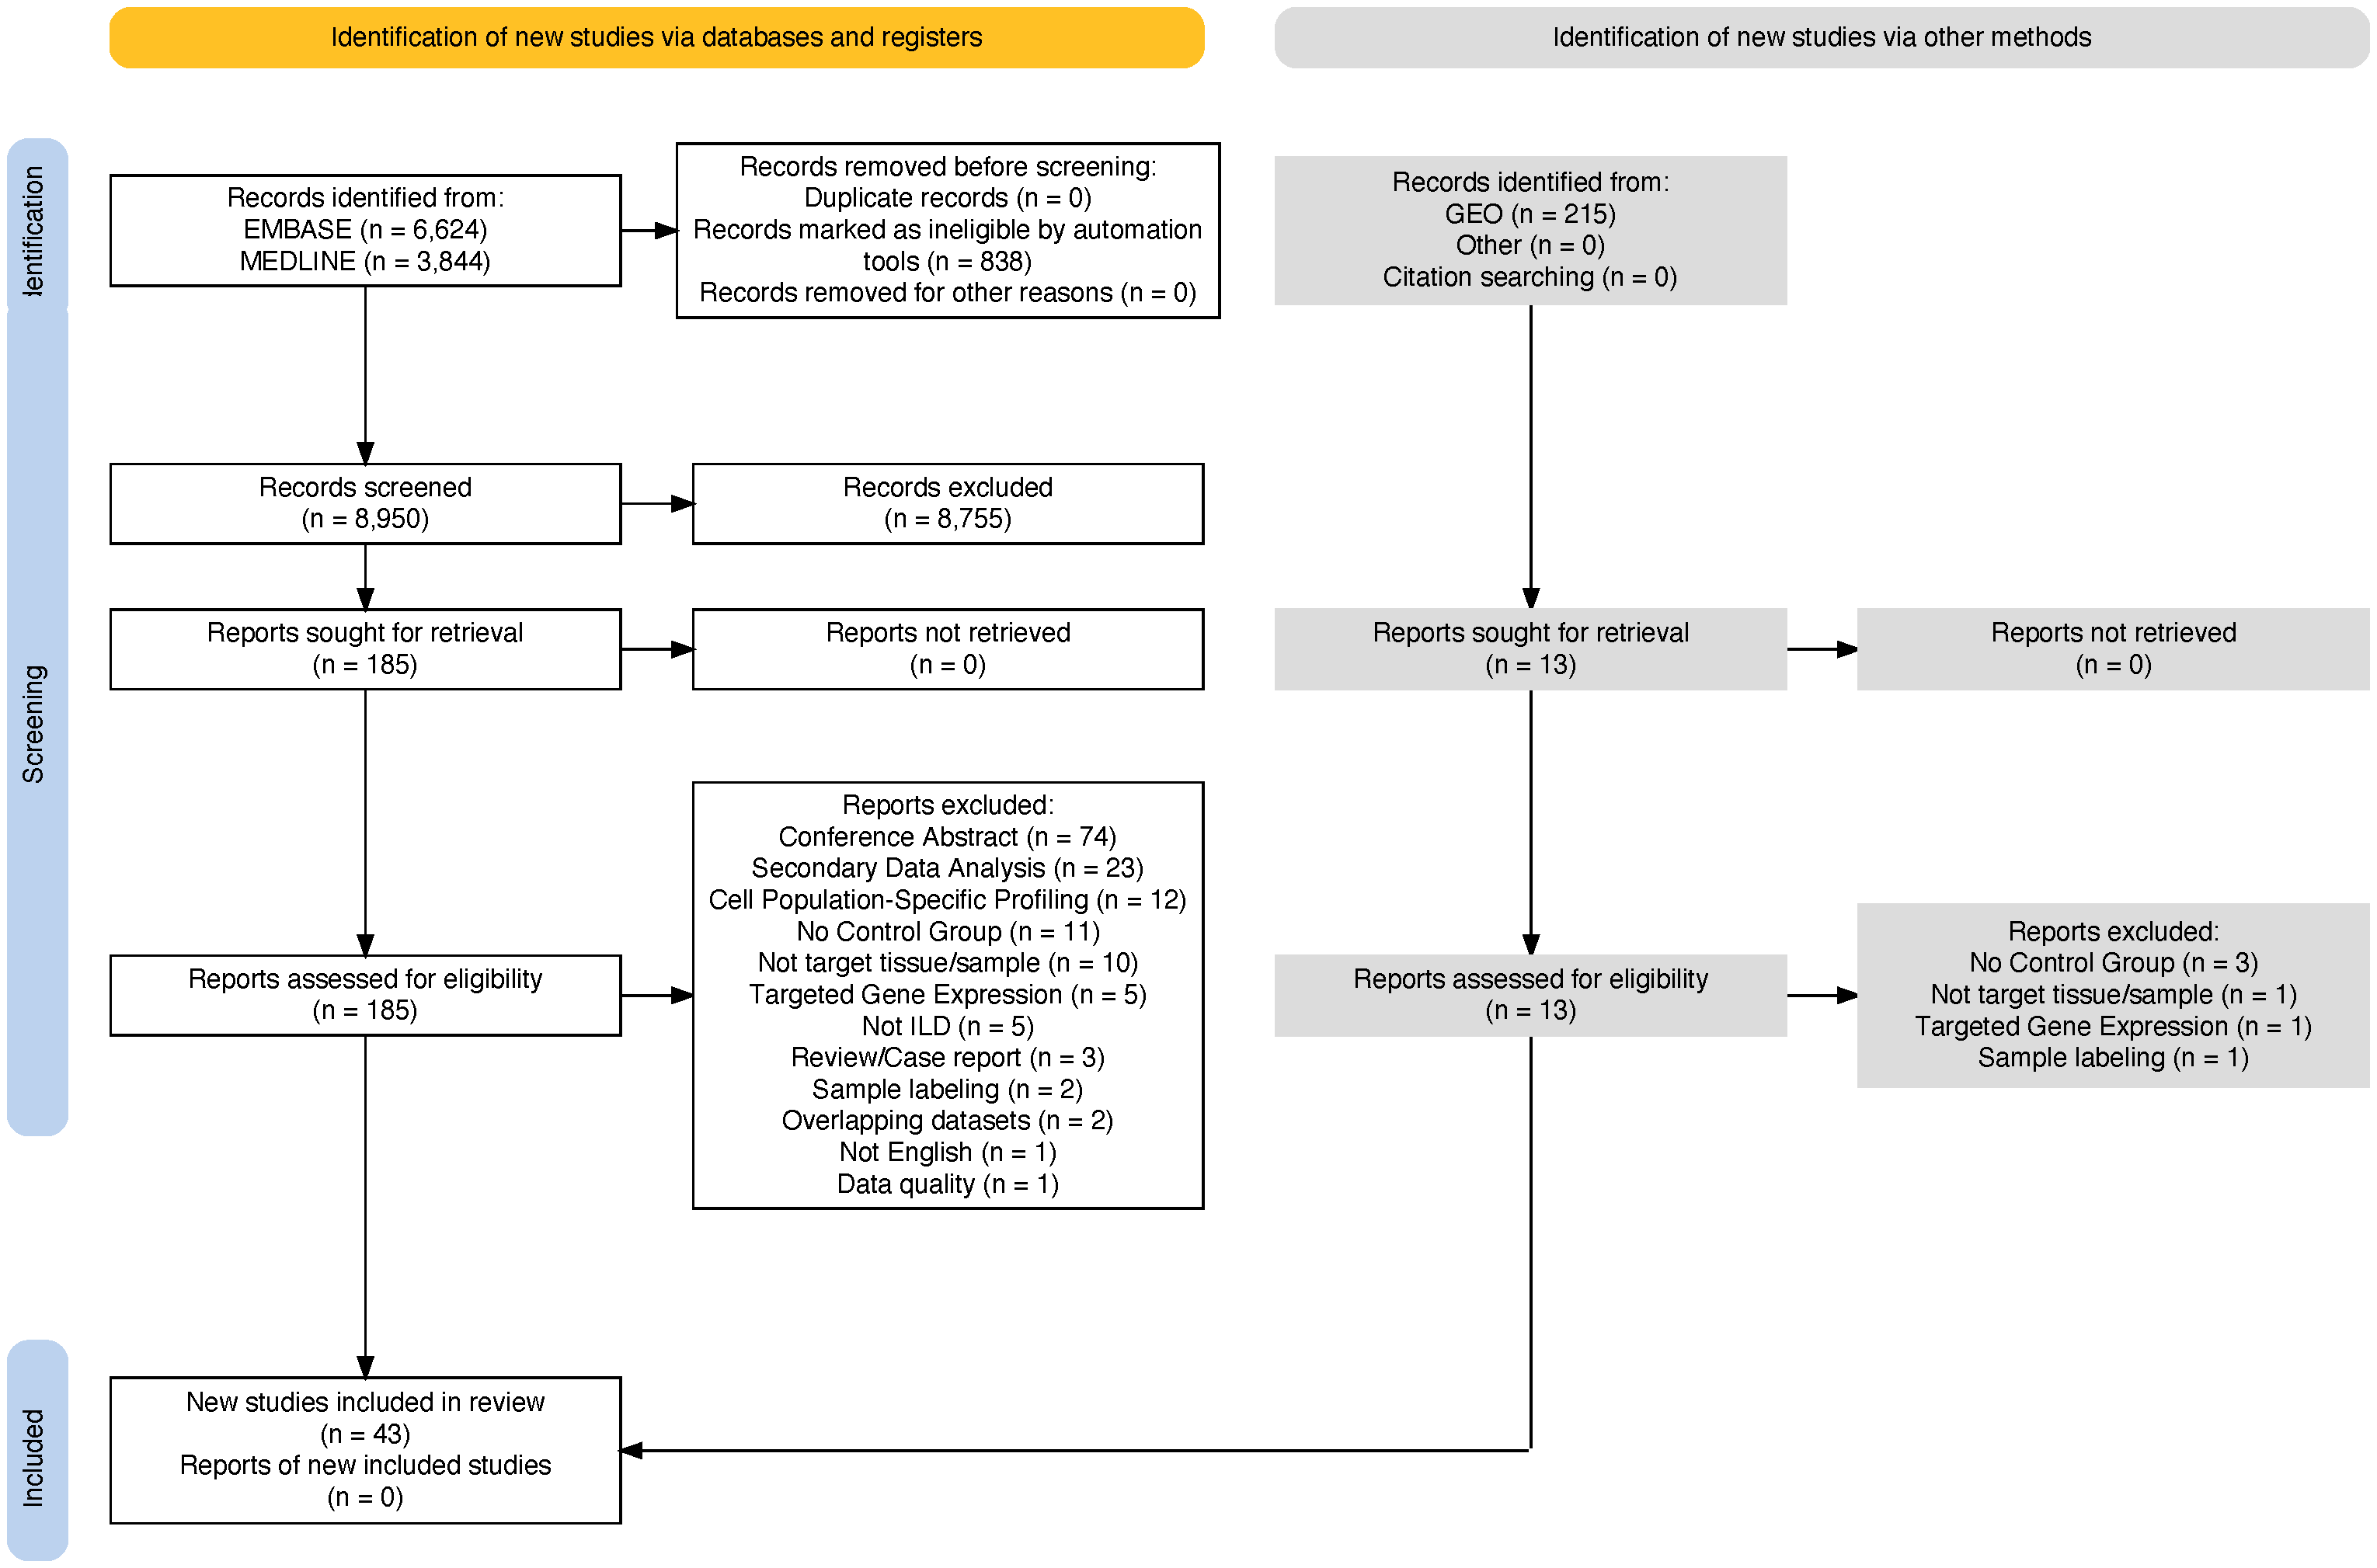
\includegraphics[width=1\linewidth,]{./Figures/Figure1_Prisma} \caption[PRISMA screening]{\textbf{Preferred Reporting Items for Systematic Reviews and Meta-Analyses (PRISMA) flowchart of study identification and screening.} MEDLINE, EMBASE, and the Gene Expression Omnibus (GEO) were examined for studies using transcriptomics to investigate samples from patients with interstitial lung disease (ILD).}\label{fig:prisma}
\end{figure}

\hypertarget{lung-gene-expression-signatures-of-fibrotic-ild-subtypes}{%
\subsubsection{Lung gene expression signatures of fibrotic ILD subtypes}\label{lung-gene-expression-signatures-of-fibrotic-ild-subtypes}}

We created lung gene signatures for each fibrotic ILD subtype via classification models generated from our MINT-integrated datasets (Figure \ref{fig:integration}). In IPF, we identified a 55-gene signature using 23 training datasets (n=576 control, n=721 IPF), which was then validated on eight test datasets (n=107 control, n=193 IPF) with AUC=0.99 {[}0.99-1.00{]} (Figure \ref{fig:mintmodel}A). To confirm the validity of MINT in identifying biologically relevant and DEGs, we compared our IPF vs Control signature against an IPF vs Control aggregate DEG list generated by RRA and found that 39 of the 55 genes were shared, including \textit{COMP}, \textit{DIO2}, \textit{MMP7} (IPF upregulated), \textit{CA4}, \textit{FAM167A}, and \textit{MYRF} (IPF downregulated) (Table E3, Figure E3A). For the peripheral transcriptome, we generated a classification model of IPF vs Control for whole blood datasets, which was validated on two PBMC datasets (AUC=0.74 {[}0.67-0.81{]}); likewise, a classification model of IPF vs Control for PBMCs was validated on two whole blood datasets (AUC=0.73 {[}0.65-0.81{]}) (Figure E4).

\newpage





































\captionsetup{width=6.5in}



\begin{table}[!h]
\centering\centering
\caption{\label{tab:datasets}\textbf{Identified lung transcriptomics studies.} Up-(\uparrow) and/or down-(\downarrow) regulated DEG lists (compared to control samples) and their location within the citation in parentheses, type of sequencing platform, GEO or SRA accession number, set assignment, and number of samples per subtype. Bolded rows indicate total sample numbers for training and test sets.}
\centering
\begin{tabu} to \linewidth {>{\raggedright\arraybackslash}p{1.35in}>{\centering\arraybackslash}p{0.9in}>{\centering\arraybackslash}p{1.15in}>{\centering\arraybackslash}p{0.5in}>{\centering\arraybackslash}p{0.3in}>{\centering\arraybackslash}p{0.3in}>{\centering\arraybackslash}p{0.3in}>{\centering\arraybackslash}p{0.6in}}
\toprule
\multicolumn{3}{c}{ } & \multicolumn{5}{c}{Number of Samples} \\
\cmidrule(l{3pt}r{3pt}){4-8}
Study & Accession & Set & Control & IPF & HP & NSIP & SSc-ILD\\
\midrule
Zuo \textit{et al.} {[}\protect\hyperlink{ref-zuo_gene_2002}{62}{]} & - & - & 4 & 3† & - & - & -\\
Pardo \textit{et al.} {[}\protect\hyperlink{ref-pardo_up-regulation_2005}{63}{]} & GSE2052 & Training & 11 & 12* & - & - & -\\
Selman \textit{et al.} {[}\protect\hyperlink{ref-selman_gene_2006}{64}{]} & - & - & 4 & 15 & 12 & 8 & -\\
Yang \textit{et al.} {[}\protect\hyperlink{ref-yang_gene_2007}{65}{]} & GSE5774 & Training & 8 & 14 & - & 2 & -\\
Bridges \textit{et al.} {[}\protect\hyperlink{ref-bridges_gene_2009}{66}{]} & - & - & 7 & 10 & - & - & -\\
Konishi \textit{et al.} {[}\protect\hyperlink{ref-konishi_gene_2009}{67}{]} & GSE10667 & Training & 15 & 23 & - & - & -\\
Rajkumar \textit{et al.} {[}\protect\hyperlink{ref-rajkumar_genomewide_2010}{68}{]} & GSE15197 & Training & 13 & 8 & - & - & -\\
Cho \textit{et al.} {[}\protect\hyperlink{ref-cho_systems_2011}{69}{]} & GSE21369 & Training & 5* & 10* & 2 & 4* & -\\
Hsu \textit{et al.} {[}\protect\hyperlink{ref-hsu_lung_2011}{70}{]} & GSE48149 & Training & 9 & 13 & - & - & 13\\
Meltzer \textit{et al.} {[}\protect\hyperlink{ref-meltzer_bayesian_2011}{71}{]} & GSE24206 & Training & 6 & 11 & - & - & -\\
Sanders \textit{et al.} {[}\protect\hyperlink{ref-sanders_altered_2012}{72}{]} & GSE35145 & Training & 4 & 4 & - & - & -\\
Deng \textit{et al.} {[}\protect\hyperlink{ref-deng_detecting_2013}{73}{]} & SRA048904 & Training & 3 & 3 & - & - & -\\
Yang \textit{et al.} {[}\protect\hyperlink{ref-yang_expression_2013}{74}{]} & GSE32537 & Training & 50 & 34 & - & 4 & -\\
Nance \textit{et al.} {[}\protect\hyperlink{ref-nance_transcriptome_2014}{75}{]} & GSE52463 & Training & 7 & 8 & - & - & -\\
Bauer \textit{et al.} {[}\protect\hyperlink{ref-bauer_novel_2015}{44}{]} & GSE47460-GPL14550 & Training & 91 & 122 & 21 & 14 & -\\
 & GSE47460-GPL6480 & Test & 17 & 38 & 9 & 3 & -\\
DePianto \textit{et al.} {[}\protect\hyperlink{ref-depianto_heterogeneous_2015}{45}{]} & GSE53845 & Test & 8 & 39 & - & - & -\\
Geng \textit{et al.} {[}\protect\hyperlink{ref-geng_down-regulation_2015}{76}{]} & GSE72073 & Training & 3 & 5 & - & - & -\\
Christmann \textit{et al.} {[}\protect\hyperlink{ref-christmann_mir-155_2016}{77}{]} & GSE81292 & Training & 5 & - & - & - & 11\\
Horimasu \textit{et al.} {[}\protect\hyperlink{ref-horimasu_clinical_2017}{78}{]} & - & - & 3 & - & 9 & - & -\\
Horimasu \textit{et al.} {[}\protect\hyperlink{ref-horimasu_gene_2017}{79}{]} & GSE101286 & Training & 3 & 7 & - & 5 & -\\
Schafer \textit{et al.} {[}\protect\hyperlink{ref-schafer_cellular_2017}{46}{]} & GSE92592 & Test & 19 & 20 & - & - & -\\
Vukmirovic \textit{et al.} {[}\protect\hyperlink{ref-vukmirovic_identification_2017}{80}{]} & GSE83717 & Training & 5 & 6 & - & - & -\\
Yu \textit{et al.} {[}\protect\hyperlink{ref-yu_reduced_2017}{47}{]} & GSE73189 & Test & 5 & 4 & - & 3 & -\\
Cecchini \textit{et al.} {[}\protect\hyperlink{ref-cecchini_comprehensive_2018}{48}{]} & GSE110147 & Test & 11 & 22 & - & 10 & -\\
Luzina \textit{et al.} {[}\protect\hyperlink{ref-luzina_transcriptomic_2018}{81}{]} & GSE99621 & Training & 3 & 3 & - & - & -\\
Sivakumar \textit{et al.} {[}\protect\hyperlink{ref-sivakumar_rna_2019}{82}{]} & GSE134692 & Training & 17 & 36 & - & - & -\\
McDonough \textit{et al.} {[}\protect\hyperlink{ref-mcdonough_transcriptional_2019}{83}{]} & GSE124685 & Training & 6 & 10 & - & - & -\\
Furusawa \textit{et al.} {[}\protect\hyperlink{ref-furusawa_chronic_2020}{84}{]} & GSE150910 & Training & 103 & 102* & 81* & - & -\\
Konigsberg \textit{et al.} {[}\protect\hyperlink{ref-konigsberg_molecular_2021}{85}{]} & GSE173355 & Training & 14 & 23 & - & - & -\\
DePianto \textit{et al.} {[}\protect\hyperlink{ref-depianto_molecular_2021}{49}{]} & GSE166036 & Test & 9 & 20 & - & - & 6\\
Borie \textit{et al.} {[}\protect\hyperlink{ref-borie_colocalization_2022}{86}{]} & GSE175457 & Training & 188 & 234 & - & - & -\\
Wang \textit{et al.} {[}\protect\hyperlink{ref-wang_canonical_2022}{87}{]} & GSE199152 & Training & 4 & 20 & - & - & -\\
Huang \textit{et al.} {[}\protect\hyperlink{ref-huang_central_2023}{88}{]} & GSE199949 & Training & 8 & 13 & - & - & -\\
De Sadeleer \textit{et al.} {[}\protect\hyperlink{ref-de_sadeleer_lung_2022}{50}{]} & GSE184316 & Test & 6 & 10 & 9 & - & -\\
Jaffar \textit{et al.} {[}\protect\hyperlink{ref-jaffar_matrix_2022}{51}{]} & GSE213001 & Test & 12 & 19 & 4 & 4 & -\\
\textbf{} & \textbf{} & \textbf{Training} & \textbf{581} & \textbf{721} & \textbf{104} & \textbf{29} & \textbf{24}\\
\textbf{} & \textbf{} & \textbf{Test} & \textbf{87} & \textbf{173} & \textbf{22} & \textbf{20} & \textbf{6}\\
\bottomrule
\multicolumn{8}{l}{\rule{0pt}{1em}\textsuperscript{*} One sample removed as an outlier}\\
\multicolumn{8}{l}{\rule{0pt}{1em}\textsuperscript{\dag} Reported as UIP}\\
\end{tabu}
\end{table}

\newpage

We applied similar strategies for the discrimination between controls, HP, SSc-ILD, and NSIP. The optimal HP vs.~Control model trained on three datasets (n=199 control, n=104 HP) had a 235-gene signature, which had an AUC of 0.91 {[}0.84-0.99{]} on the test datasets (n=35 control, n=22 HP) (Figure \ref{fig:mintmodel}B). For SSc-ILD, the model trained on two datasets (n=14 control, n=24 SSc-ILD) contained 52 genes, which was validated on the test dataset (n=9 control, n=6 SSc-ILD) with an AUC of 0.98 (0.93-1.00) in distinguishing SSc-ILD from control samples (Figure \ref{fig:mintmodel}C). The best-performing NSIP vs.~Control model trained on five datasets (n=157 control, n=29 NSIP) had a 378-gene signature, which was validated on four test datasets (n=45 control, n=20 NSIP) with an AUC of 0.94 {[}0.88-0.99{]} (Figure \ref{fig:mintmodel}D). Model performance on individual datasets and cumulative performance can be found in Table \ref{tab:modelPerf}, and a list of gene signatures and model weights can be found in Table E4.



\begin{figure}
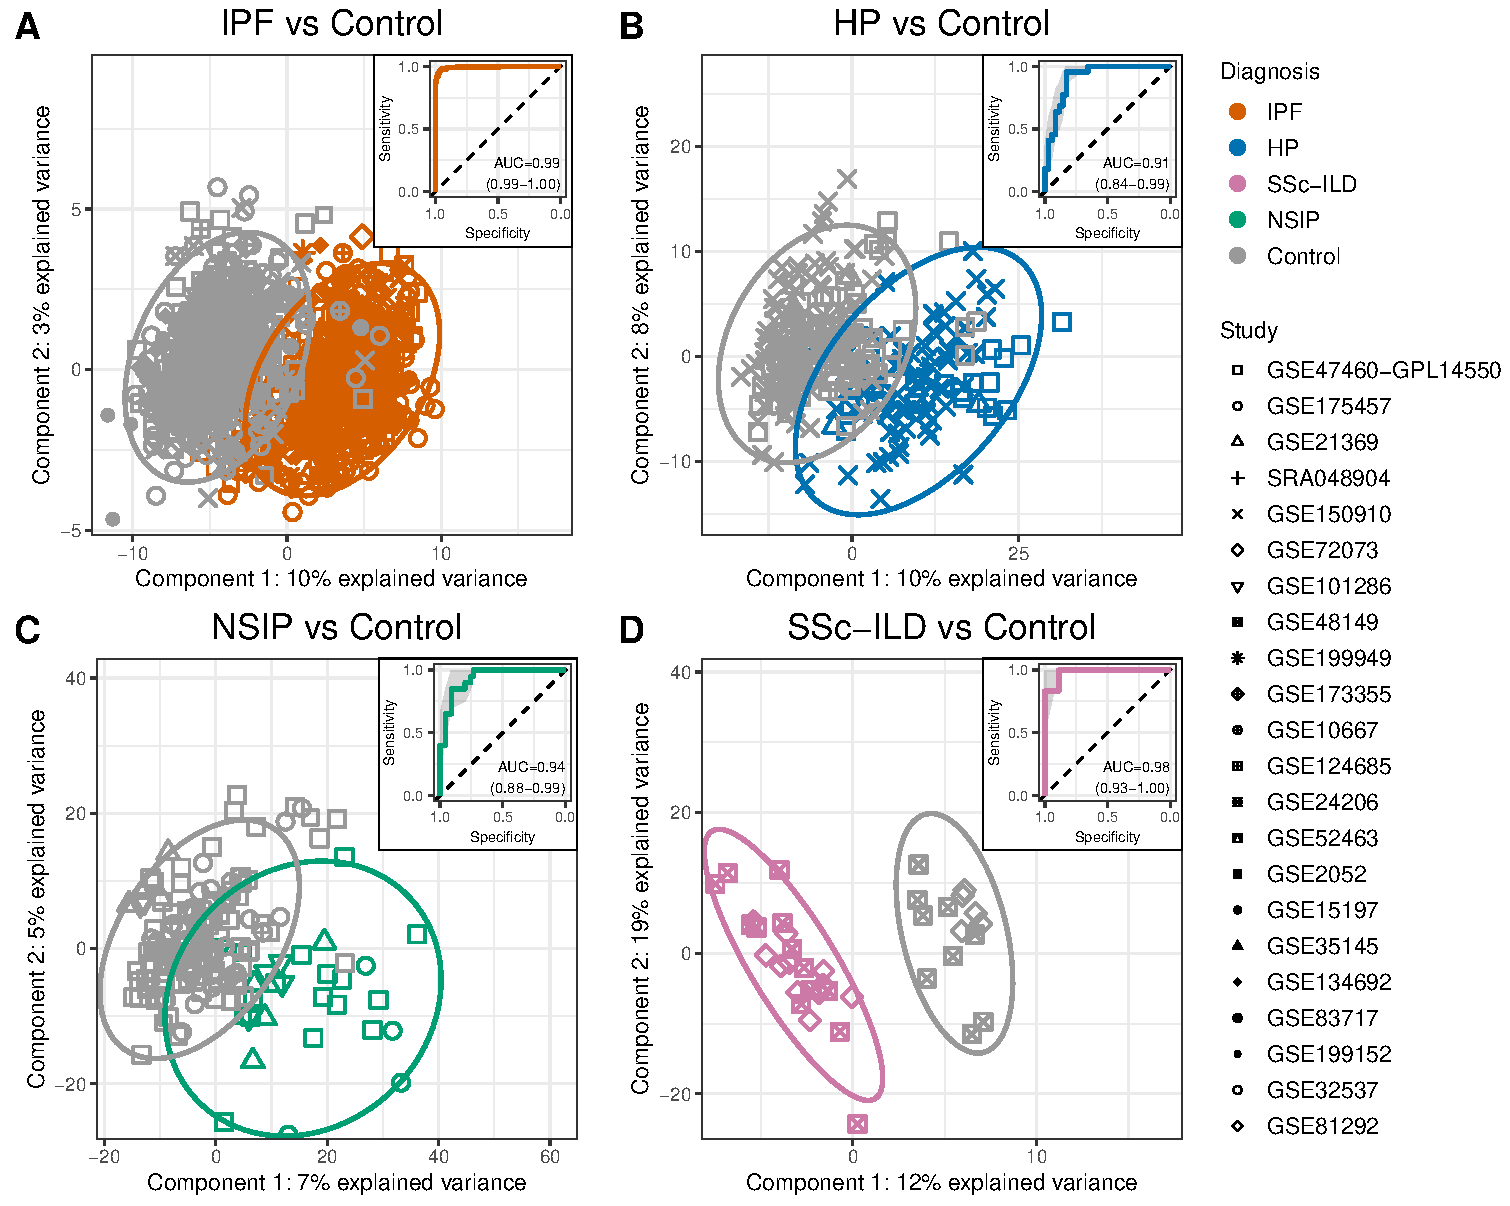
\includegraphics[width=1\linewidth,]{./Figures/Figure3_MINT} \caption[MINT models]{\textbf{Classification models for ILD subtypes against controls.} Training set datasets were integrated and tuned to develop classification models, which were then validated on test set datasets. Projection of MINT-integrated training set samples into the space of the first two PLS components for IPF (A), HP (B), SSc-ILD (C), and NSIP (D) classification models. Inset: AUC performance of each ILD classification model on held-out test datasets. Detailed performance metrics for each dataset can be found in Table \ref{tab:modelPerf}.}\label{fig:mintmodel}
\end{figure}

The same methodology was used to perform sex-specific analyses for IPF, HP, and NSIP by inferring sex from expression of sex-specific genes. All of our sex-specific models had comparable performance between the test set of the same sex and the opposite sex, with the exception of the male NSIP classification model (male test set: AUC=0.98 {[}0.93-1.00{]}; female test set: AUC=0.79 {[}0.68-0.90) (Table \ref{tab:sexModel}). Pathway analysis using genes uniquely identified in each sex-specific model revealed an overrepresentation of immune-related pathways in females and fibrosis-related pathways in males (Table E6, Table E7).

\hypertarget{fibrotic-ild-subtypes-are-differentiated-at-the-transcriptional-level}{%
\subsubsection{Fibrotic ILD subtypes are differentiated at the transcriptional level}\label{fibrotic-ild-subtypes-are-differentiated-at-the-transcriptional-level}}

To examine identifying features of fibrotic ILD subtypes at the transcriptional level, we generated classification models for IPF, HP, and NSIP against all other ILD subtypes. Our training set consisted of 721 IPF, 104 HP, 29 NSIP, 24 SSc-ILD, 14 RB-ILD, 14 unknown fibrosis, six COP, four DIP, three rheumatoid arthritis-ILD (RA-ILD), and one CTD-ILD samples, while our test set consisted of 193 IPF, 22 HP, 20 NSIP, six SSc-ILD, five mixed IPF-NSIP, three unknown fibrosis, two RB-ILD, two DIP, two CTD-ILD, one COP, and one combined pulmonary fibrosis and emphysema (CPFE) samples. The 57-gene IPF vs other ILD model trained on seven datasets had good performance on the six test datasets (AUC=0.71 {[}0.63-0.79{]}), as did the 132-gene HP vs other ILD model trained on three datasets on the two test datasets (AUC=0.76 {[}0.63-0.89{]}) (Figure \ref{fig:ILDvILD}. Our NSIP vs other ILD model trained on five datasets did not have a good performance on four test datasets (AUC=0.60 {[}0.49-0.72{]}) (Figure \ref{fig:nsipmodel}. For between-subtype comparisons, we identified a 95-gene signature differentiating IPF from HP samples, which had an AUC of 0.76 (0.64-0.87) on three test datasets, as well as a 67-gene signature differentiating IPF from NSIP samples, which had an AUC of 0.76 (0.64-0.88) on four test datasets (Figure \ref{fig:ildvsildspecific}A-D). A classifier differentiating HP from NSIP had variable performance on 2 test datasets (AUC=0.74 {[}0.51-0.96{]}) (Figure \ref{fig:ildvsildspecific}E, F).



\begin{figure}
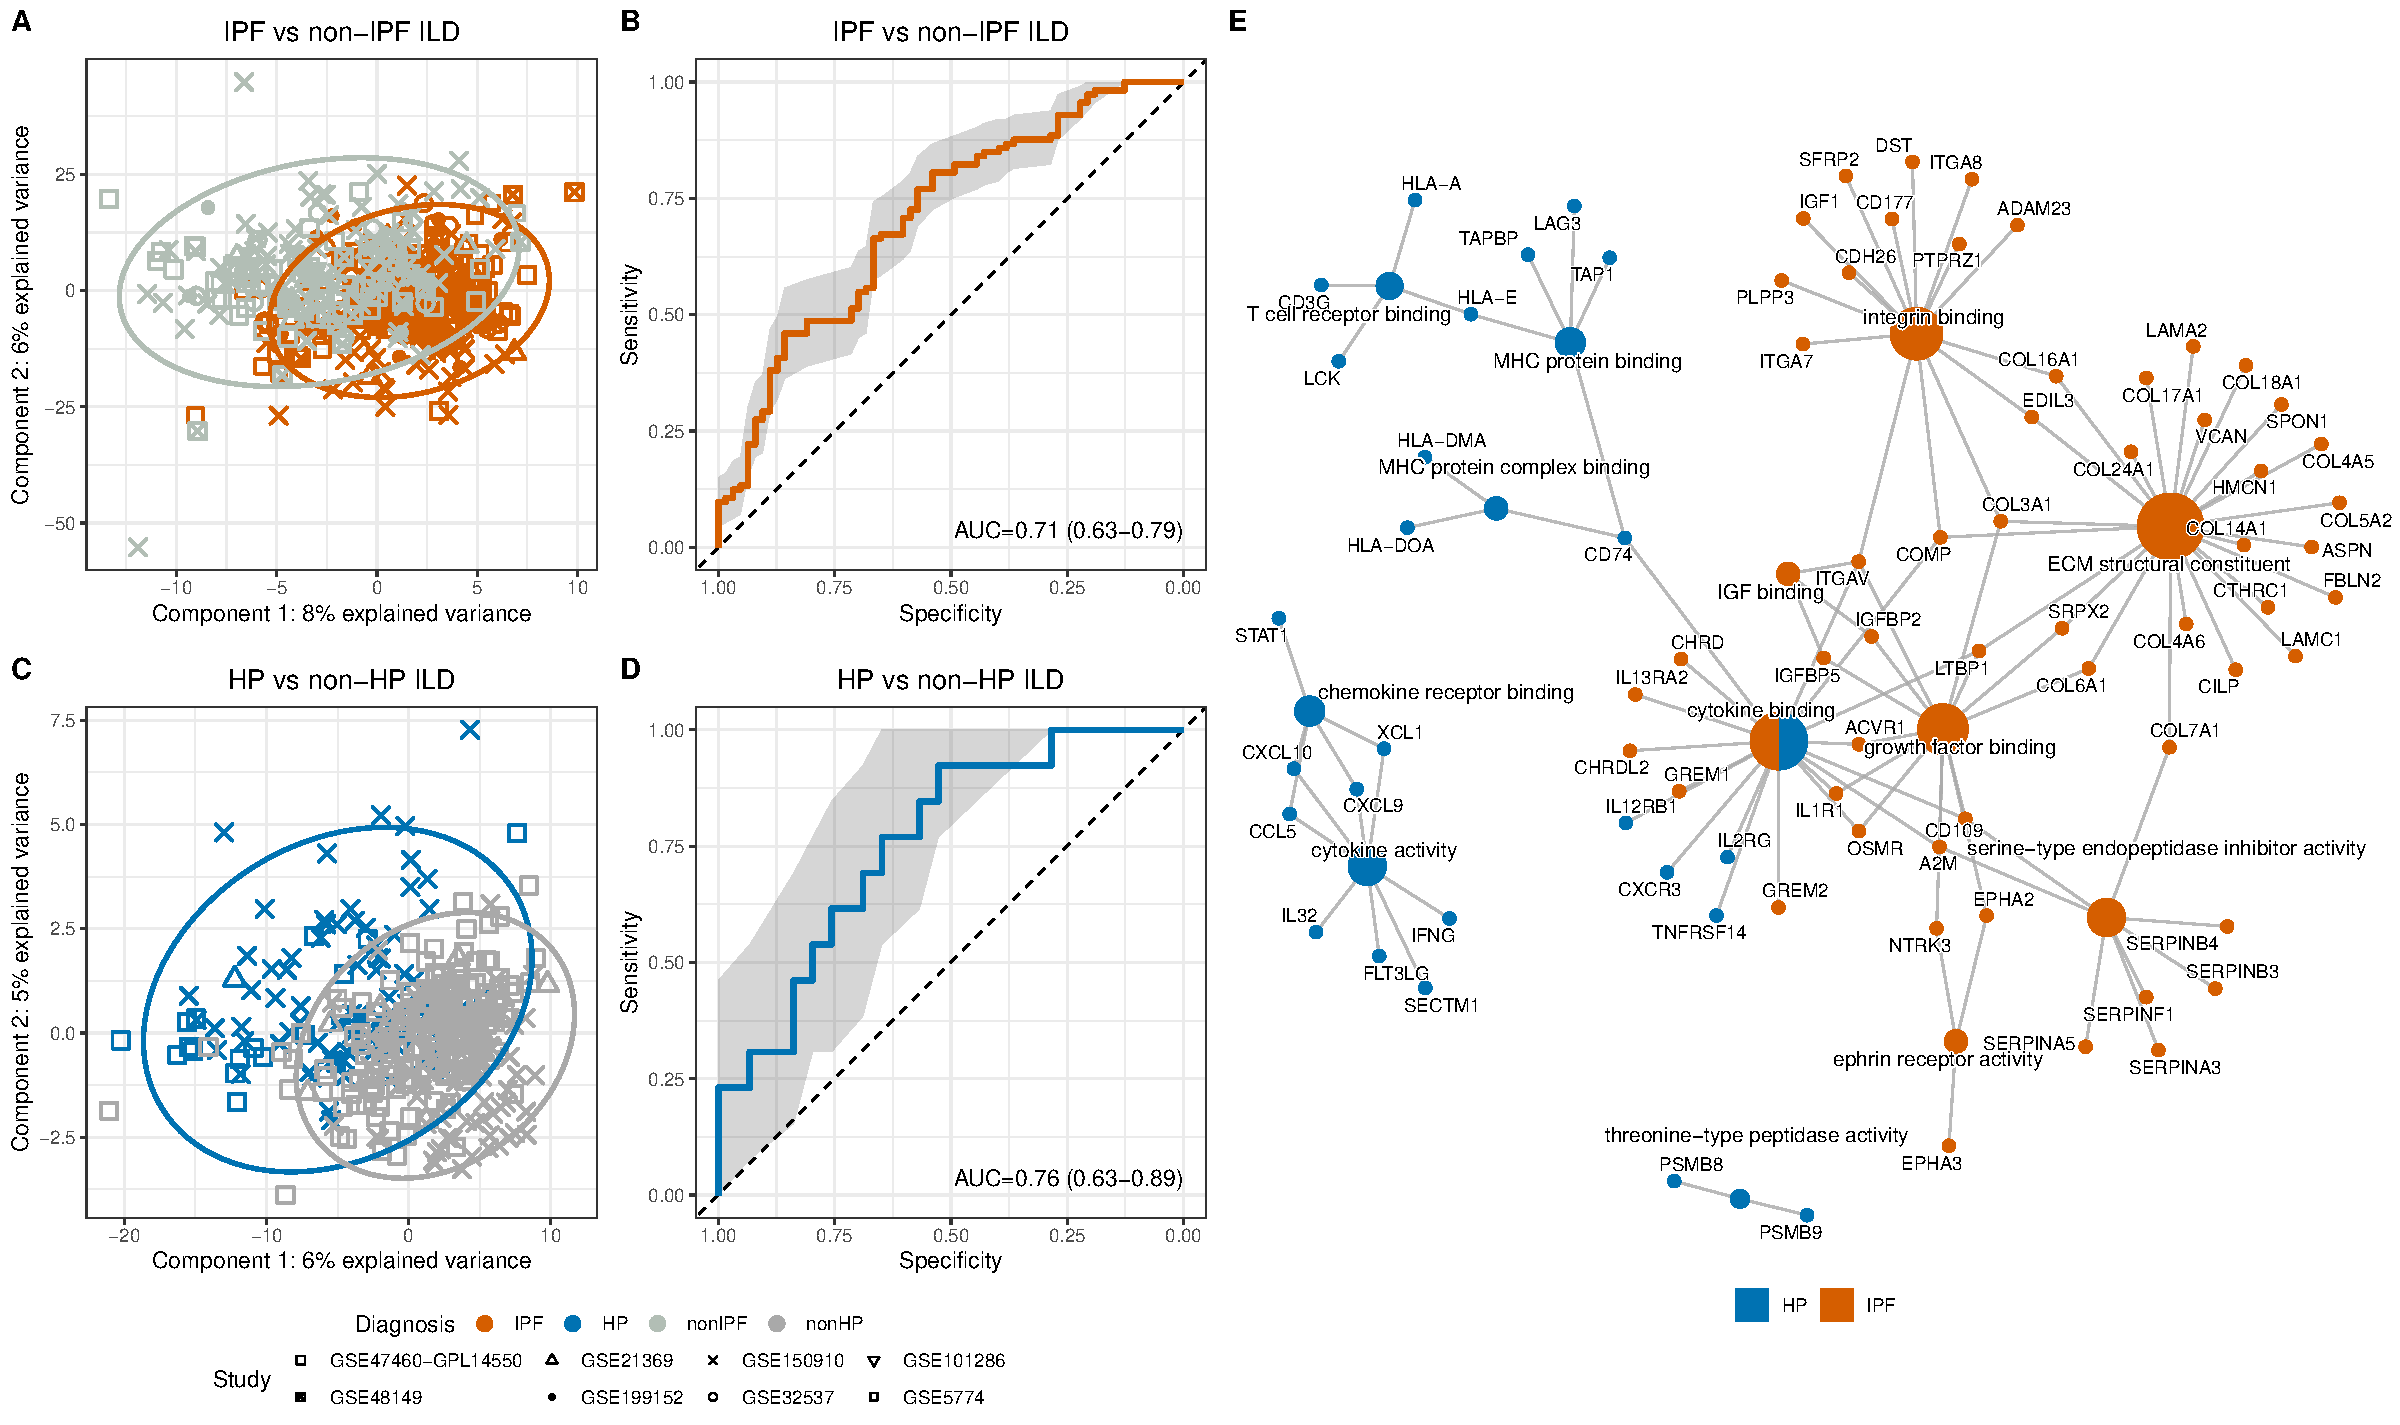
\includegraphics[width=1\linewidth,]{./Figures/Figure4_ILDvsILD} \caption[ILD vs ILD]{\textbf{ILD subtype-specific classification models.} IPF-specific and HP-specific classification models were developed through MINT integration of lung transcriptomics datasets. MINT-PLS projection of samples for classification models of IPF vs non-IPF ILD (A) and HP vs non-HP ILD (C), with corresponding performance on held-out test datasets (B, D). Upregulated gene ontology pathways using gene signatures identified in classification models for IPF against non-IPF ILD and HP against non-HP ILD are shown in E.}\label{fig:ILDvILD}
\end{figure}

\hypertarget{ild-subtypes-have-both-common-and-unique-disease-pathways}{%
\subsubsection{ILD subtypes have both common and unique disease pathways}\label{ild-subtypes-have-both-common-and-unique-disease-pathways}}

As the ILD classification models had few genes for pathway analysis, we generated ``expanded'' classification models with an increased number of genes using Bayesian changepoint analysis and verified their discrimination ability using the same test sets (Figure E7, Table E8). Using the expanded gene signatures for Gene Ontology (GO) overrepresentation analysis of ILD subtypes against controls, we identified \textit{MMP7}, \textit{COMP}, \textit{DIO2}, \textit{THBS4}, \textit{IL13RA2}, \textit{MEOX1}, \{COL17A1\}, and \{SCG5\} as shared upregulated genes across all subtypes when compared against controls (Figure \ref{fig:ILDpathways}A, Figure E3C, Table E4). With reference to the MSigDB C8 collection and a manually curated database of single-cell RNA-seq annotations obtained from previous pulmonary fibrosis publications, these genes are primarily expressed by aberrant basaloid and basal cells (Figure \ref{fig:ILDpathways}C, Table E9). Shared downregulated genes suggested a decrease in AT1 (\textit{MYRF}, \textit{AGER}) and endothelial (\textit{CA4}, \textit{PRX}, \textit{VIPR1}) cells (Figure @ref\{fig:ILDpathways\}B, Figure E3D). No genes in the signatures for the lung IPF vs Control model were shared with peripheral signatures; however, blood and PBMC gene signatures shared 21 genes (Figure E3B).



\begin{figure}
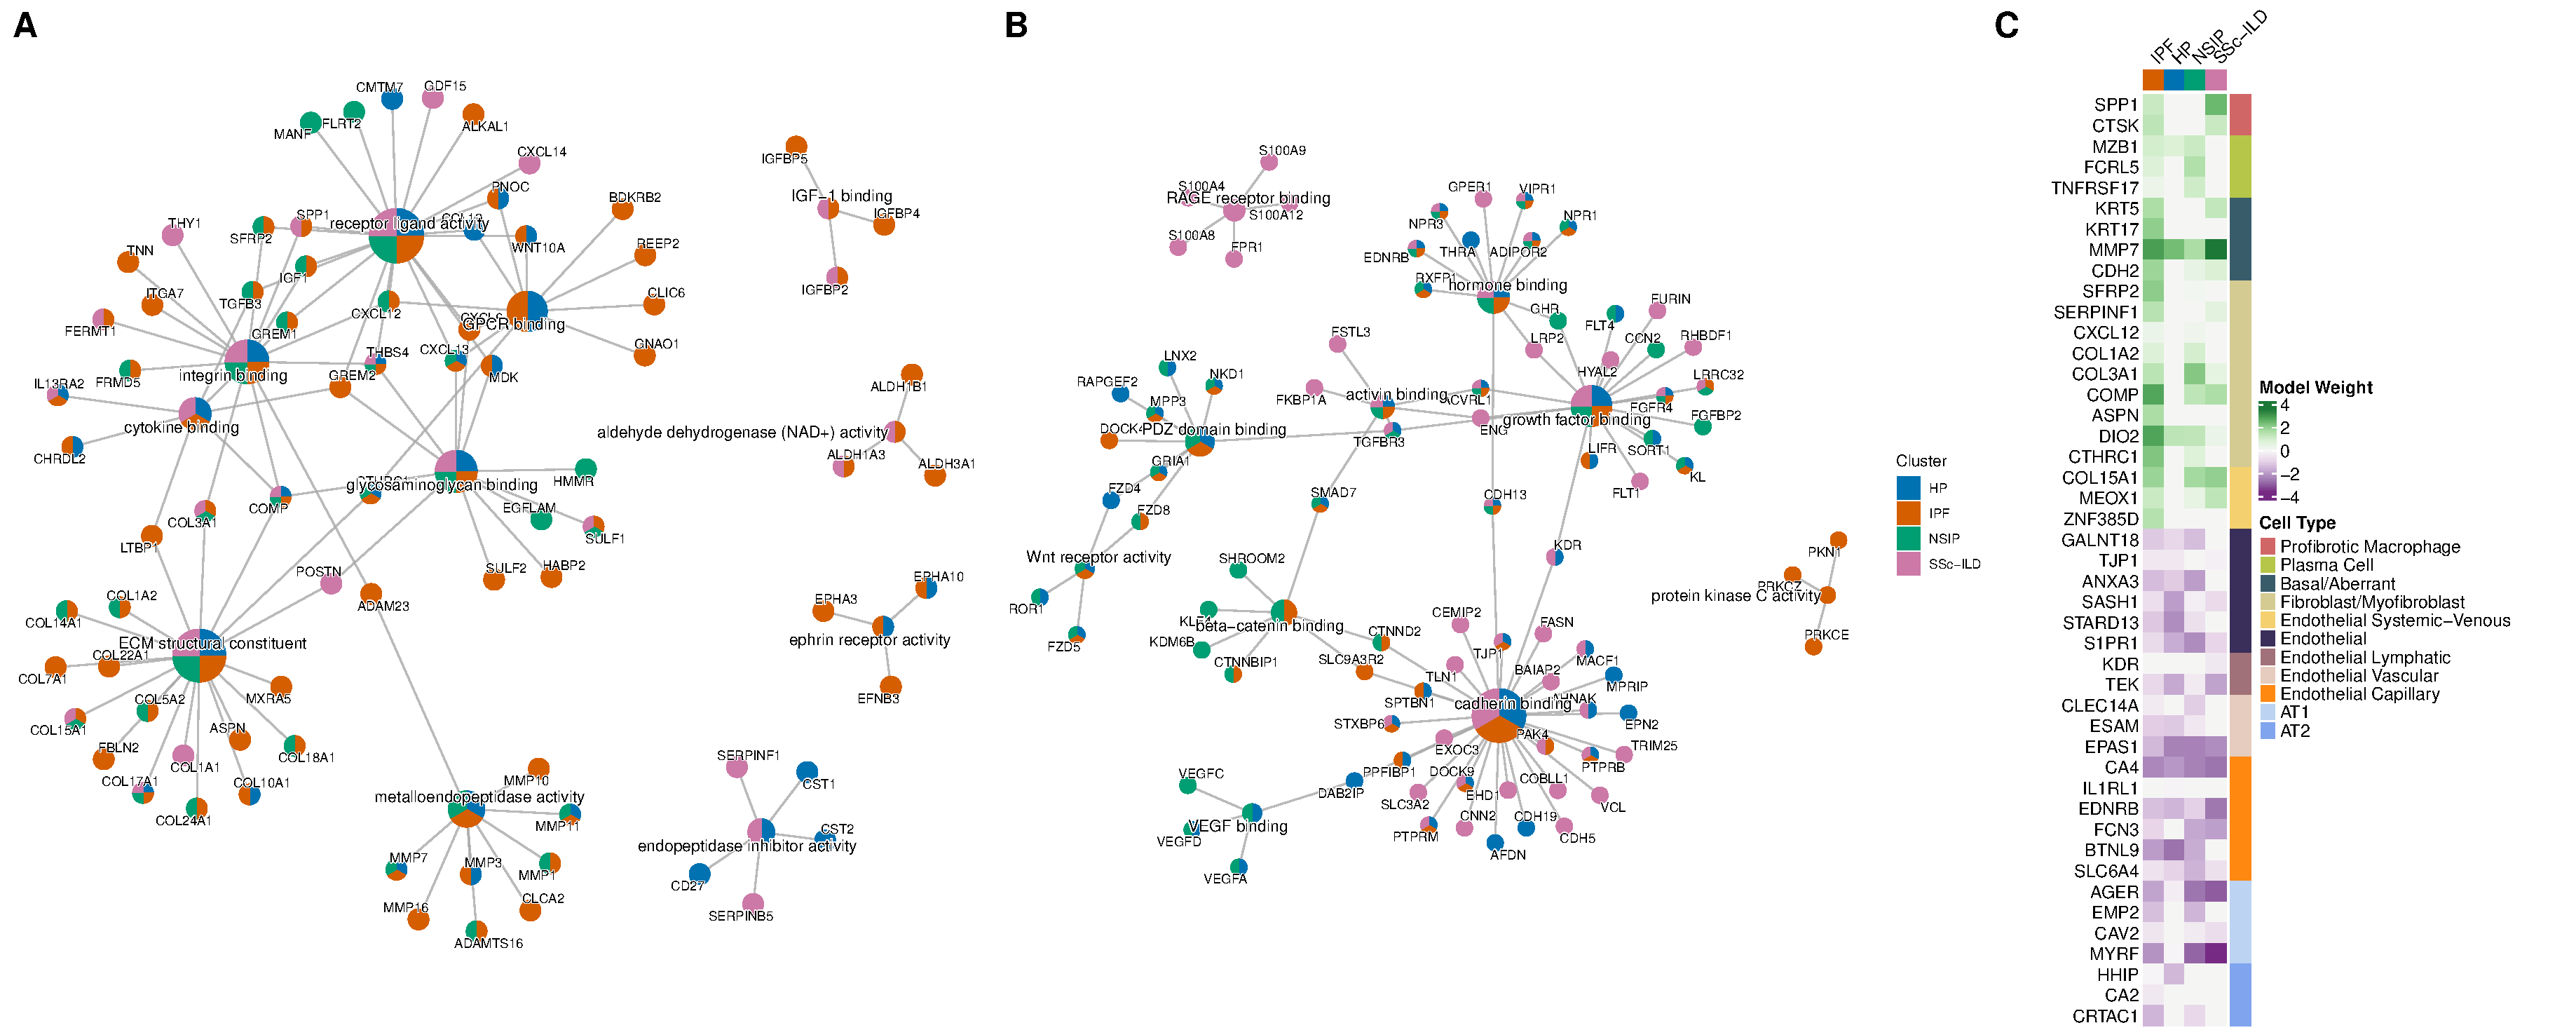
\includegraphics[width=1\linewidth,]{./Figures/Figure5_pathways} \caption[ILD pathways]{\textbf{Pathway analysis of gene signatures from classification models of ILD subtypes against control.} Using up- (A) and down-regulated (B) gene signatures from each ILD classification model, overrepresentation analysis of gene ontology (GO) terms was performed and visualized as a gene-concept network plot. (C) A heatmap of model weights for selected gene markers associated with single-cell marker annotations identified in ILD scRNA-seq analysis (see Data Supplement).}\label{fig:ILDpathways}
\end{figure}

When comparing IPF against other ILD subtypes, we identified GPSM2, HSPA4L (previously shown to be involved in the differentiation of AT2 cells (56)), and ECM-related genes such as COL16A1, ITGA7, and VCAN as uniquely upregulated in IPF (Table E8). In HP, we identified antigen presentation and major histocompatibility complex (MHC) binding as enriched pathways via PSMB8, PSMB9, and TAPBP expression (Figure 4E), and these genes were also included in the models differentiating HP from IPF and NSIP samples. When compared to controls, SSc-ILD samples were uniquely characterized by expression of CDH3, which encodes E-cadherin and was not found to be upregulated in signatures of other fibrotic ILD subtypes.
Unsupervised analysis identifies putative molecular endotypes of ILD
We next used biclustering, an unsupervised learning method, to examine transcriptomic lung samples for specific molecular endotypes. Biclustering algorithms perform simultaneous clustering of rows (genes) and columns (samples) of a data matrix to identify subsets known as biclusters (19). We extracted all studies containing lung gene expression data, performed batch correction, and used a series of biclustering algorithms to identify 16 biclusters showing enrichment in specific lung disease groups (Figure E8, Figure E9). Pathway analysis of bicluster genes revealed associations with lung cell types and fibrosis, and top results were used to annotate each bicluster (Table E10, Figure 6A,B). Of the samples with available predicted FVC\% and DLCO\% data, we identified IPF samples in the `M13-Proliferation' bicluster (n=53) as having lower FVC\% compared to non-cluster (n=155) IPF samples (-6.29\%, FDR=0.09) (Figure 6C), which we confirmed was not due to age (-1.18 years, p=0.15). ILD samples in the `U4-AT1 cells', `U0-Endothelium', `M2-Cytoskeleton', `U1-EMT', `M9-Fibrosis', and `M13-Proliferation' biclusters had significantly lower DLCO\% (-7.95 to -13.9\%, all FDR\textless0.05) compared to non-cluster samples, though these samples were all significantly older with the exception of the `M13-Proliferation' samples which were younger (-2.18 years, FDR=9.17×10-3). A full list of results can be found in Table E11.

\hypertarget{this-could-be-a-sub-hedding}{%
\subsection{This could be a sub-hedding}\label{this-could-be-a-sub-hedding}}

Lorem ipsum dolor sit amet, consectetur adipiscing elit. Nulla eleifend odio odio, et consectetur nunc commodo vitae. Donec eu finibus lacus. Integer at porta nulla. Fusce dignissim gravida lacinia. Nulla ut odio in ante imperdiet placerat. Maecenas vel imperdiet lorem. Proin ultricies, ex at bibendum fringilla, neque libero malesuada sem, in tincidunt leo mi vel mi. Phasellus scelerisque sagittis urna sed sodales. Curabitur iaculis justo velit, ultricies euismod justo convallis non. Nunc id purus et ante iaculis dignissim vel non erat. Donec dignissim urna ut lobortis congue. Nulla tempus ut ipsum non ornare. Donec ac purus nec sem cursus eleifend. Suspendisse potenti. Vestibulum ac vehicula ante.

\hypertarget{in-text-citations}{%
\subsection{In-text citations}\label{in-text-citations}}

Read section \href{https://bookdown.org/yihui/bookdown/citations.html}{2.8} of the bookdown guide for more details.

To use in-text citations like this {[}\protect\hyperlink{ref-degoede2017}{\textbf{degoede2017?}}{]}, add bibliographic entries to the \emph{References/reference\_list.bib} file, then you can reference the entries using the \emph{citation key}: \texttt{{[}@key{]}} e.g.~\texttt{{[}@degoede2017{]}}.

UBCdown comes with two reference styles: Harvard, and Vancouver. To change styles, just edit the YAML section of \texttt{main\_script.Rmd} to reference the appropriate \texttt{.csl} file. If desired, you can also add/replace with your own citation style file \texttt{.csl}.

\hypertarget{referencing-figures}{%
\subsection{Referencing figures}\label{referencing-figures}}

\hypertarget{basics}{%
\subsubsection{Basics}\label{basics}}

This text will render with a figure referenced (Figure \ref{fig:figureTitle}).

\begin{figure}

\includegraphics{main_script_files/figure-latex/figureTitle-1} \caption[This is the short title for the figure list]{This is the long caption of the figure that will apear in the main text.}\label{fig:figureTitle}
\end{figure}

\hypertarget{text-references-for-figure-captions}{%
\subsubsection{Text-references for figure captions}\label{text-references-for-figure-captions}}

You may need to use citations or special characters in a figure caption, which is not possible by writing the caption directly in the code chunk \texttt{fig.cap} option. Instead, you will need to use \href{https://bookdown.org/yihui/bookdown/markdown-extensions-by-bookdown.html\#text-references}{in-text references}.

How to use in-text references:

\begin{enumerate}
\def\labelenumi{\arabic{enumi}.}
\tightlist
\item
  in the \texttt{fig.cap} code chunk option, write \texttt{"(ref:TEXT-REFERENCE)"}
\item
  outside of code chunk (in the text), start a paragraph with \texttt{(ref:TEXT-REFERENCE)\ ...} then write your caption
\end{enumerate}

Note: ``TEXT-REFERENCE'' can be replace with whatever, I suggest something descriptive like ``figureTitle-cap''



\begin{figure}

\includegraphics{main_script_files/figure-latex/figureTitle-22-1} \caption[This is the short title for the figure list]{This caption was written with an in-text reference. See how I can use citations like this {[}\protect\hyperlink{ref-degoede2017}{\textbf{degoede2017?}}{]} and \textbf{special} \emph{characters} \_!?@\#, which normally would not be possible.}\label{fig:figureTitle-22}
\end{figure}

\hypertarget{tables}{%
\subsection{Tables}\label{tables}}

Tables are best generated by using \texttt{kable} + \texttt{kableExtra} (Table \ref{tab:IntroTable1}). These R packages allow for a lot of customization. I suggest saving your tables as \texttt{.csv} files and then loading them into R with \texttt{readr::read\_csv}.

\captionsetup{width=6.5in}

\begin{table}[!h]
\centering\centering
\caption{\label{tab:IntroTable1}This is the title of the table.}
\centering
\begin{tabu} to \linewidth {>{\raggedright}X>{\raggedright}X>{\raggedleft}X>{\raggedleft}X>{\raggedleft}X}
\toprule
GEO Accession & Primary groups & African & Asian & Caucasian\\
\midrule
GSE98224 & EOPET & 5 & 4 & 10\\
 & Preterm Controls & 1 & 3 & 5\\
 & LOPET & 1 & 1 & 8\\
 & Term Controls & 0 & 4 & 5\\
GSE71678 & NA* & 0 & 0 & 342\\
\bottomrule
\multicolumn{5}{l}{\rule{0pt}{1em}EOPET - Early Onset Preeclampsia.}\\
\multicolumn{5}{l}{\rule{0pt}{1em}\textsuperscript{*} Can add footnotes here.}\\
\end{tabu}
\end{table}

See \href{https://bookdown.org/yihui/bookdown/tables.html}{2.5} for details. Tables are referenced in the same way as figures, through the code chunk label. The title of the table is specified in the \texttt{caption} option under the \texttt{kableExtra::kbl} call.

\clearpage

\hypertarget{insert-title-of-chapter-3-here}{%
\section{Insert Title of Chapter 3 Here}\label{insert-title-of-chapter-3-here}}

\renewcommand{\thefigure}{3.\arabic{figure}}
\setcounter{figure}{0}
\renewcommand{\thetable}{3.\arabic{table}}
\setcounter{table}{0}
\renewcommand{\theequation}{3.\arabic{equation}}
\setcounter{equation}{0}

\clearpage

\hypertarget{insert-title-of-chapter-4-here}{%
\section{Insert Title of Chapter 4 Here}\label{insert-title-of-chapter-4-here}}

\renewcommand{\thefigure}{4.\arabic{figure}}
\setcounter{figure}{0}
\renewcommand{\thetable}{4.\arabic{table}}
\setcounter{table}{0}
\renewcommand{\theequation}{4.\arabic{equation}}
\setcounter{equation}{0}

\clearpage

\hypertarget{insert-title-of-chapter-5-here}{%
\section{Insert Title of Chapter 5 Here}\label{insert-title-of-chapter-5-here}}

\renewcommand{\thefigure}{5.\arabic{figure}}
\setcounter{figure}{0}
\renewcommand{\thetable}{5.\arabic{table}}
\setcounter{table}{0}
\renewcommand{\theequation}{5.\arabic{equation}}
\setcounter{equation}{0}

\clearpage

\hypertarget{conclusion}{%
\section{Conclusion}\label{conclusion}}

Lorem ipsum dolor sit amet, consectetur adipiscing elit. Cras id nulla malesuada, auctor arcu at, tempor nibh. Etiam ultricies dictum nisi eu vulputate. Suspendisse tempor aliquam efficitur. Curabitur eget orci ac purus hendrerit laoreet. Proin porta arcu nisl, a fermentum tellus suscipit et. Nulla mattis orci ac tortor facilisis venenatis. Phasellus a velit tristique, tincidunt purus id, aliquet tellus. Orci varius natoque penatibus et magnis dis parturient montes, nascetur ridiculus mus. Sed et turpis sed odio faucibus aliquam nec eget est.

Phasellus ligula lacus, euismod posuere pretium sit amet, ornare condimentum nisl. Integer eu aliquet lectus, sit amet sagittis turpis. Etiam tempus bibendum nibh, eu accumsan sapien. Suspendisse tincidunt sit amet nisi vel consectetur. Donec vitae odio elit. Quisque dignissim risus feugiat nunc tempor hendrerit. Fusce consequat lectus eget felis tempus, et lobortis ante ornare. Etiam euismod quam eu scelerisque mattis. Praesent nisi lectus, tincidunt nec sapien ac, fermentum pellentesque orci.

Praesent semper faucibus mauris, in suscipit quam mattis et. Curabitur malesuada placerat magna. Morbi eget bibendum purus, sollicitudin faucibus enim. Donec condimentum arcu quis eros placerat sodales. Nunc non elit sodales, blandit risus vel, mattis odio. Nullam in aliquet ligula, ut viverra enim. Aliquam viverra justo non neque consequat dictum. Nunc tempor arcu sem, non blandit nisl dapibus eu. Donec vitae pretium magna. Nam risus augue, ultricies ac sollicitudin ut, rutrum eleifend purus. Donec lorem turpis, lacinia quis pretium non, sollicitudin eu enim. Curabitur eu eros congue, vehicula ante vitae, semper elit.

Fusce feugiat consectetur erat, nec venenatis massa malesuada nec. Curabitur varius convallis sem eget efficitur. Morbi congue odio non turpis cursus efficitur. In hac habitasse platea dictumst. Cras porttitor porttitor nibh id tempor. Sed bibendum quam nisl, sed congue lectus condimentum et. Curabitur nec mauris sapien. Morbi dictum ex sodales turpis ornare mattis. Suspendisse potenti. Pellentesque commodo lorem purus, id mattis nibh efficitur et. Cras tempus rutrum interdum. Vestibulum ante ipsum primis in faucibus orci luctus et ultrices posuere cubilia curae; Mauris placerat ligula eu nisl sagittis consequat. Curabitur placerat, elit quis cursus tempor, mauris augue posuere metus, ut elementum orci diam maximus lectus. Proin sed sodales nulla. Maecenas non sapien nec mauris facilisis fringilla.

\clearpage

\section*{Bibliography}
\addcontentsline{toc}{section}{Bibliography}

\noindent
\leftskip=2em
\parindent=-2em

\hypertarget{refs}{}
\begin{CSLReferences}{0}{0}
\leavevmode\vadjust pre{\hypertarget{ref-raghu_diagnosis_2018}{}}%
\CSLLeftMargin{1. }%
\CSLRightInline{Raghu G, Remy-Jardin M, Myers JL, Richeldi L, Ryerson CJ, Lederer DJ, et al. \href{https://doi.org/10.1164/rccm.201807-1255ST}{Diagnosis of {Idiopathic} {Pulmonary} {Fibrosis}. {An} {Official} {ATS}/{ERS}/{JRS}/{ALAT} {Clinical} {Practice} {Guideline}}. American Journal of Respiratory and Critical Care Medicine. 2018 Sep;198(5):e44--68. }

\leavevmode\vadjust pre{\hypertarget{ref-raghu_idiopathic_2022}{}}%
\CSLLeftMargin{2. }%
\CSLRightInline{Raghu G, Remy-Jardin M, Richeldi L, Thomson CC, Inoue Y, Johkoh T, et al. Idiopathic {Pulmonary} {Fibrosis} (an {Update}) and {Progressive} {Pulmonary} {Fibrosis} in {Adults}: {An} {Official} {ATS}/{ERS}/{JRS}/{ALAT} {Clinical} {Practice} {Guideline}. American Journal of Respiratory and Critical Care Medicine {[}Internet{]}. 2022 May {[}cited 2023 Jan 5{]};205(9):e18--47. Available from: \url{https://www.atsjournals.org/doi/full/10.1164/rccm.202202-0399ST}}

\leavevmode\vadjust pre{\hypertarget{ref-hopkins_epidemiology_2016}{}}%
\CSLLeftMargin{3. }%
\CSLRightInline{Hopkins RB, Burke N, Fell C, Dion G, Kolb M. \href{https://doi.org/10.1183/13993003.01504-2015}{Epidemiology and survival of idiopathic pulmonary fibrosis from national data in {Canada}}. The European Respiratory Journal. 2016 Jul;48(1):187--95. }

\leavevmode\vadjust pre{\hypertarget{ref-canadian_cancer_statistics_advisory_committee_in_collaboration_with_the_canadian_cancer_society_statistics_canada_and_the_public_health_agency_of_canada_canadian_2023}{}}%
\CSLLeftMargin{4. }%
\CSLRightInline{Canadian Cancer Statistics Advisory Committee in collaboration with the Canadian Cancer Society, Statistics Canada and the Public Health Agency of Canada. Canadian {Cancer} {Statistics} 2023 {[}Internet{]}. Toronto, ON: Canadian Cancer Society; 2023 {[}cited 2024 May 18{]}. Available from: \url{https://cancer.ca/en/research/cancer-statistics/canadian-cancer-statistics}}

\leavevmode\vadjust pre{\hypertarget{ref-raghu_comorbidities_2015}{}}%
\CSLLeftMargin{5. }%
\CSLRightInline{Raghu G, Amatto VC, Behr J, Stowasser S. \href{https://doi.org/10.1183/13993003.02316-2014}{Comorbidities in idiopathic pulmonary fibrosis patients: A systematic literature review}. The European Respiratory Journal. 2015 Oct;46(4):1113--30. }

\leavevmode\vadjust pre{\hypertarget{ref-morell_treatment_2016}{}}%
\CSLLeftMargin{6. }%
\CSLRightInline{Morell F, Esser D, Lim J, Stowasser S, Villacampa A, Nieves D, et al. \href{https://doi.org/10.1186/s12890-016-0168-6}{Treatment patterns, resource use and costs of idiopathic pulmonary fibrosis in {Spain}--results of a {Delphi} {Panel}}. BMC pulmonary medicine. 2016 Jan;16:7. }

\leavevmode\vadjust pre{\hypertarget{ref-hilberg_economic_2018}{}}%
\CSLLeftMargin{7. }%
\CSLRightInline{Hilberg O, Bendstrup E, Ibsen R, Løkke A, Hyldgaard C. \href{https://doi.org/10.1183/23120541.00045-2017}{Economic consequences of idiopathic pulmonary fibrosis in {Denmark}}. ERJ open research. 2018 Apr;4(2):00045--2017. }

\leavevmode\vadjust pre{\hypertarget{ref-ley_clinical_2011}{}}%
\CSLLeftMargin{8. }%
\CSLRightInline{Ley B, Collard HR, King TE. Clinical {Course} and {Prediction} of {Survival} in {Idiopathic} {Pulmonary} {Fibrosis}. American Journal of Respiratory and Critical Care Medicine {[}Internet{]}. 2011 Feb {[}cited 2023 May 2{]};183(4):431--40. Available from: \url{https://www.atsjournals.org/doi/10.1164/rccm.201006-0894CI}}

\leavevmode\vadjust pre{\hypertarget{ref-bagnato_cellular_2015}{}}%
\CSLLeftMargin{9. }%
\CSLRightInline{Bagnato G, Harari S. \href{https://doi.org/10.1183/09059180.00003214}{Cellular interactions in the pathogenesis of interstitial lung diseases}. European Respiratory Review: An Official Journal of the European Respiratory Society. 2015 Mar;24(135):102--14. }

\leavevmode\vadjust pre{\hypertarget{ref-marconi_epithelial-mesenchymal_2021}{}}%
\CSLLeftMargin{10. }%
\CSLRightInline{Marconi GD, Fonticoli L, Rajan TS, Pierdomenico SD, Trubiani O, Pizzicannella J, et al. Epithelial-{Mesenchymal} {Transition} ({EMT}): {The} {Type}-2 {EMT} in {Wound} {Healing}, {Tissue} {Regeneration} and {Organ} {Fibrosis}. Cells {[}Internet{]}. 2021 Jun {[}cited 2024 May 19{]};10(7):1587. Available from: \url{https://www.ncbi.nlm.nih.gov/pmc/articles/PMC8307661/}}

\leavevmode\vadjust pre{\hypertarget{ref-byrne_pulmonary_2015}{}}%
\CSLLeftMargin{11. }%
\CSLRightInline{Byrne AJ, Mathie SA, Gregory LG, Lloyd CM. \href{https://doi.org/10.1136/thoraxjnl-2015-207020}{Pulmonary macrophages: Key players in the innate defence of the airways}. Thorax. 2015 Dec;70(12):1189--96. }

\leavevmode\vadjust pre{\hypertarget{ref-zhu_m2_2017}{}}%
\CSLLeftMargin{12. }%
\CSLRightInline{Zhu L, Fu X, Chen X, Han X, Dong P. \href{https://doi.org/10.1002/cbin.10788}{M2 macrophages induce {EMT} through the {TGF}-β/{Smad2} signaling pathway}. Cell Biology International. 2017 Sep;41(9):960--8. }

\leavevmode\vadjust pre{\hypertarget{ref-lederer_idiopathic_2018}{}}%
\CSLLeftMargin{13. }%
\CSLRightInline{Lederer DJ, Martinez FJ. Idiopathic {Pulmonary} {Fibrosis}. New England Journal of Medicine {[}Internet{]}. 2018 May {[}cited 2022 Apr 21{]};378(19):1811--23. Available from: \url{https://doi.org/10.1056/NEJMra1705751}}

\leavevmode\vadjust pre{\hypertarget{ref-idiopathic_pulmonary_fibrosis_clinical_research_network_prednisone_2012}{}}%
\CSLLeftMargin{14. }%
\CSLRightInline{Idiopathic Pulmonary Fibrosis Clinical Research Network, Raghu G, Anstrom KJ, King TE, Lasky JA, Martinez FJ. \href{https://doi.org/10.1056/NEJMoa1113354}{Prednisone, azathioprine, and {N}-acetylcysteine for pulmonary fibrosis}. The New England Journal of Medicine. 2012 May;366(21):1968--77. }

\leavevmode\vadjust pre{\hypertarget{ref-lynch_diagnostic_2018}{}}%
\CSLLeftMargin{15. }%
\CSLRightInline{Lynch DA, Sverzellati N, Travis WD, Brown KK, Colby TV, Galvin JR, et al. \href{https://doi.org/10.1016/S2213-2600(17)30433-2}{Diagnostic criteria for idiopathic pulmonary fibrosis: A {Fleischner} {Society} {White} {Paper}}. The Lancet Respiratory Medicine. 2018 Feb;6(2):138--53. }

\leavevmode\vadjust pre{\hypertarget{ref-walsh_multicentre_2016}{}}%
\CSLLeftMargin{16. }%
\CSLRightInline{Walsh SLF, Wells AU, Desai SR, Poletti V, Piciucchi S, Dubini A, et al. \href{https://doi.org/10.1016/S2213-2600(16)30033-9}{Multicentre evaluation of multidisciplinary team meeting agreement on diagnosis in diffuse parenchymal lung disease: A case-cohort study}. The Lancet Respiratory Medicine. 2016 Jul;4(7):557--65. }

\leavevmode\vadjust pre{\hypertarget{ref-graney_interstitial_2019}{}}%
\CSLLeftMargin{17. }%
\CSLRightInline{Graney BA, Fischer A. \href{https://doi.org/10.1513/AnnalsATS.201808-565CME}{Interstitial {Pneumonia} with {Autoimmune} {Features}}. Annals of the American Thoracic Society. 2019 May;16(5):525--33. }

\leavevmode\vadjust pre{\hypertarget{ref-skolnik_unclassifiable_2016}{}}%
\CSLLeftMargin{18. }%
\CSLRightInline{Skolnik K, Ryerson CJ. \href{https://doi.org/10.1111/resp.12568}{Unclassifiable interstitial lung disease: {A} review}. Respirology (Carlton, Vic). 2016 Jan;21(1):51--6. }

\leavevmode\vadjust pre{\hypertarget{ref-flaherty_nintedanib_2019}{}}%
\CSLLeftMargin{19. }%
\CSLRightInline{Flaherty KR, Wells AU, Cottin V, Devaraj A, Walsh SLF, Inoue Y, et al. Nintedanib in {Progressive} {Fibrosing} {Interstitial} {Lung} {Diseases}. New England Journal of Medicine {[}Internet{]}. 2019 Oct {[}cited 2023 Aug 5{]};381(18):1718--27. Available from: \url{https://doi.org/10.1056/NEJMoa1908681}}

\leavevmode\vadjust pre{\hypertarget{ref-maher_pirfenidone_2020}{}}%
\CSLLeftMargin{20. }%
\CSLRightInline{Maher TM, Corte TJ, Fischer A, Kreuter M, Lederer DJ, Molina-Molina M, et al. \href{https://doi.org/10.1016/S2213-2600(19)30341-8}{Pirfenidone in patients with unclassifiable progressive fibrosing interstitial lung disease: A double-blind, randomised, placebo-controlled, phase 2 trial}. The Lancet Respiratory Medicine. 2020 Feb;8(2):147--57. }

\leavevmode\vadjust pre{\hypertarget{ref-behr_pirfenidone_2021}{}}%
\CSLLeftMargin{21. }%
\CSLRightInline{Behr J, Prasse A, Kreuter M, Johow J, Rabe KF, Bonella F, et al. Pirfenidone in patients with progressive fibrotic interstitial lung diseases other than idiopathic pulmonary fibrosis ({RELIEF}): A double-blind, randomised, placebo-controlled, phase 2b trial. The Lancet Respiratory Medicine {[}Internet{]}. 2021 May {[}cited 2024 May 20{]};9(5):476--86. Available from: \url{https://www.sciencedirect.com/science/article/pii/S2213260020305543}}

\leavevmode\vadjust pre{\hypertarget{ref-khor_patient_2023}{}}%
\CSLLeftMargin{22. }%
\CSLRightInline{Khor YH, Farooqi M, Hambly N, Kolb M, Ryerson CJ, Assayag D, et al. Patient {Characteristics} and {Survival} for {Progressive} {Pulmonary} {Fibrosis} {Using} {Different} {Definitions}. American Journal of Respiratory and Critical Care Medicine {[}Internet{]}. 2023 Jan {[}cited 2024 May 20{]};207(1):102--5. Available from: \url{https://www.atsjournals.org/doi/10.1164/rccm.202205-0910LE}}

\leavevmode\vadjust pre{\hypertarget{ref-nasser_progressive_2021}{}}%
\CSLLeftMargin{23. }%
\CSLRightInline{Nasser M, Larrieu S, Si-Mohamed S, Ahmad K, Boussel L, Brevet M, et al. \href{https://doi.org/10.1183/13993003.02718-2020}{Progressive fibrosing interstitial lung disease: A clinical cohort (the {PROGRESS} study)}. The European Respiratory Journal. 2021 Feb;57(2):2002718. }

\leavevmode\vadjust pre{\hypertarget{ref-takei_prevalence_2022}{}}%
\CSLLeftMargin{24. }%
\CSLRightInline{Takei R, Brown KK, Yamano Y, Kataoka K, Yokoyama T, Matsuda T, et al. \href{https://doi.org/10.1111/resp.14245}{Prevalence and prognosis of chronic fibrosing interstitial lung diseases with a progressive phenotype}. Respirology (Carlton, Vic). 2022 May;27(5):333--40. }

\leavevmode\vadjust pre{\hypertarget{ref-hambly_prevalence_2022}{}}%
\CSLLeftMargin{25. }%
\CSLRightInline{Hambly N, Farooqi MM, Dvorkin-Gheva A, Donohoe K, Garlick K, Scallan C, et al. \href{https://doi.org/10.1183/13993003.02571-2021}{Prevalence and characteristics of progressive fibrosing interstitial lung disease in a prospective registry}. The European Respiratory Journal. 2022 Oct;60(4):2102571. }

\leavevmode\vadjust pre{\hypertarget{ref-oldham_lung_2022-1}{}}%
\CSLLeftMargin{26. }%
\CSLRightInline{Oldham JM, Lee CT, Wu Z, Bowman WS, Pugashetti JV, Dao N, et al. \href{https://doi.org/10.1183/13993003.01396-2021}{Lung function trajectory in progressive fibrosing interstitial lung disease}. The European Respiratory Journal. 2022 Jun;59(6):2101396. }

\leavevmode\vadjust pre{\hypertarget{ref-rajan_progressive_2023}{}}%
\CSLLeftMargin{27. }%
\CSLRightInline{Rajan SK, Cottin V, Dhar R, Danoff S, Flaherty KR, Brown KK, et al. Progressive pulmonary fibrosis: An expert group consensus statement. European Respiratory Journal {[}Internet{]}. 2023 Mar {[}cited 2024 May 20{]};61(3). Available from: \url{https://erj.ersjournals.com/content/61/3/2103187}}

\leavevmode\vadjust pre{\hypertarget{ref-cosgrove_barriers_2018}{}}%
\CSLLeftMargin{28. }%
\CSLRightInline{Cosgrove GP, Bianchi P, Danese S, Lederer DJ. Barriers to timely diagnosis of interstitial lung disease in the real world: The {INTENSITY} survey. BMC Pulmonary Medicine {[}Internet{]}. 2018 Jan {[}cited 2022 Apr 22{]};18:9. Available from: \url{https://www.ncbi.nlm.nih.gov/pmc/articles/PMC5773175/}}

\leavevmode\vadjust pre{\hypertarget{ref-grewal_role_2019}{}}%
\CSLLeftMargin{29. }%
\CSLRightInline{Grewal JS, Morisset J, Fisher JH, Churg AM, Bilawich AM, Ellis J, et al. \href{https://doi.org/10.1513/AnnalsATS.201811-794OC}{Role of a {Regional} {Multidisciplinary} {Conference} in the {Diagnosis} of {Interstitial} {Lung} {Disease}}. Annals of the American Thoracic Society. 2019 Apr;16(4):455--62. }

\leavevmode\vadjust pre{\hypertarget{ref-lamas_delayed_2011}{}}%
\CSLLeftMargin{30. }%
\CSLRightInline{Lamas DJ, Kawut SM, Bagiella E, Philip N, Arcasoy SM, Lederer DJ. \href{https://doi.org/10.1164/rccm.201104-0668OC}{Delayed access and survival in idiopathic pulmonary fibrosis: A cohort study}. American Journal of Respiratory and Critical Care Medicine. 2011 Oct;184(7):842--7. }

\leavevmode\vadjust pre{\hypertarget{ref-drakopanagiotakis_biomarkers_2018}{}}%
\CSLLeftMargin{31. }%
\CSLRightInline{Drakopanagiotakis F, Wujak L, Wygrecka M, Markart P. \href{https://doi.org/10.1016/j.matbio.2018.01.023}{Biomarkers in idiopathic pulmonary fibrosis}. Matrix Biology: Journal of the International Society for Matrix Biology. 2018 Aug;68-69:404--21. }

\leavevmode\vadjust pre{\hypertarget{ref-morais_serum_2015}{}}%
\CSLLeftMargin{32. }%
\CSLRightInline{Morais A, Beltrão M, Sokhatska O, Costa D, Melo N, Mota P, et al. \href{https://doi.org/10.1016/j.rmed.2015.06.003}{Serum metalloproteinases 1 and 7 in the diagnosis of idiopathic pulmonary fibrosis and other interstitial pneumonias}. Respiratory Medicine. 2015 Aug;109(8):1063--8. }

\leavevmode\vadjust pre{\hypertarget{ref-vukmirovic_impact_2018}{}}%
\CSLLeftMargin{33. }%
\CSLRightInline{Vukmirovic M, Kaminski N. Impact of {Transcriptomics} on {Our} {Understanding} of {Pulmonary} {Fibrosis}. Frontiers in Medicine {[}Internet{]}. 2018 Apr {[}cited 2023 May 2{]};5:87. Available from: \url{https://www.ncbi.nlm.nih.gov/pmc/articles/PMC5894436/}}

\leavevmode\vadjust pre{\hypertarget{ref-khan_systematic_2022}{}}%
\CSLLeftMargin{34. }%
\CSLRightInline{Khan FA, Stewart I, Saini G, Robinson KA, Jenkins RG. \href{https://doi.org/10.1183/13993003.01612-2021}{A systematic review of blood biomarkers with individual participant data meta-analysis of matrix metalloproteinase-7 in idiopathic pulmonary fibrosis}. The European Respiratory Journal. 2022 Apr;59(4):2101612. }

\leavevmode\vadjust pre{\hypertarget{ref-white_plasma_2016}{}}%
\CSLLeftMargin{35. }%
\CSLRightInline{White ES, Xia M, Murray S, Dyal R, Flaherty CM, Flaherty KR, et al. \href{https://doi.org/10.1164/rccm.201505-0862OC}{Plasma {Surfactant} {Protein}-{D}, {Matrix} {Metalloproteinase}-7, and {Osteopontin} {Index} {Distinguishes} {Idiopathic} {Pulmonary} {Fibrosis} from {Other} {Idiopathic} {Interstitial} {Pneumonias}}. American Journal of Respiratory and Critical Care Medicine. 2016 Nov;194(10):1242--51. }

\leavevmode\vadjust pre{\hypertarget{ref-spagnolo_early_2021}{}}%
\CSLLeftMargin{36. }%
\CSLRightInline{Spagnolo P, Ryerson CJ, Putman R, Oldham J, Salisbury M, Sverzellati N, et al. Early diagnosis of fibrotic interstitial lung disease: Challenges and opportunities. The Lancet Respiratory Medicine {[}Internet{]}. 2021 Sep {[}cited 2023 May 2{]};9(9):1065--76. Available from: \url{https://www.thelancet.com/journals/lanres/article/PIIS2213-2600(21)00017-5/fulltext}}

\leavevmode\vadjust pre{\hypertarget{ref-johannson_treatment_2021}{}}%
\CSLLeftMargin{37. }%
\CSLRightInline{Johannson KA, Chaudhuri N, Adegunsoye A, Wolters PJ. Treatment of fibrotic interstitial lung disease: Current approaches and future directions. The Lancet {[}Internet{]}. 2021 Oct {[}cited 2023 May 2{]};398(10309):1450--60. Available from: \url{https://www.thelancet.com/journals/lancet/article/PIIS0140-6736(21)01826-2/fulltext}}

\leavevmode\vadjust pre{\hypertarget{ref-pankratz_usual_2017}{}}%
\CSLLeftMargin{38. }%
\CSLRightInline{Pankratz DG, Choi Y, Imtiaz U, Fedorowicz GM, Anderson JD, Colby TV, et al. \href{https://doi.org/10.1513/AnnalsATS.201612-947OC}{Usual {Interstitial} {Pneumonia} {Can} {Be} {Detected} in {Transbronchial} {Biopsies} {Using} {Machine} {Learning}}. Annals of the American Thoracic Society. 2017 Nov;14(11):1646--54. }

\leavevmode\vadjust pre{\hypertarget{ref-choi_analytical_2017}{}}%
\CSLLeftMargin{39. }%
\CSLRightInline{Choi Y, Lu J, Hu Z, Pankratz DG, Jiang H, Cao M, et al. Analytical performance of {Envisia}: A genomic classifier for usual interstitial pneumonia. BMC Pulmonary Medicine {[}Internet{]}. 2017 Nov {[}cited 2023 May 2{]};17:141. Available from: \url{https://www.ncbi.nlm.nih.gov/pmc/articles/PMC5693488/}}

\leavevmode\vadjust pre{\hypertarget{ref-dupuy_critical_2007}{}}%
\CSLLeftMargin{40. }%
\CSLRightInline{Dupuy A, Simon RM. \href{https://doi.org/10.1093/jnci/djk018}{Critical review of published microarray studies for cancer outcome and guidelines on statistical analysis and reporting}. Journal of the National Cancer Institute. 2007 Jan;99(2):147--57. }

\leavevmode\vadjust pre{\hypertarget{ref-rohart_mint_2017}{}}%
\CSLLeftMargin{41. }%
\CSLRightInline{Rohart F, Eslami A, Matigian N, Bougeard S, Lê Cao KA. {MINT}: A multivariate integrative method to identify reproducible molecular signatures across independent experiments and platforms. BMC Bioinformatics {[}Internet{]}. 2017 Feb {[}cited 2023 Jan 12{]};18(1):128. Available from: \url{https://doi.org/10.1186/s12859-017-1553-8}}

\leavevmode\vadjust pre{\hypertarget{ref-rohart_mixomics_2017}{}}%
\CSLLeftMargin{42. }%
\CSLRightInline{Rohart F, Gautier B, Singh A, Cao KAL. {mixOmics}: {An} {R} package for `omics feature selection and multiple data integration. PLOS Computational Biology {[}Internet{]}. 2017 Nov {[}cited 2023 Dec 18{]};13(11):e1005752. Available from: \url{https://journals.plos.org/ploscompbiol/article?id=10.1371/journal.pcbi.1005752}}

\leavevmode\vadjust pre{\hypertarget{ref-kolde_robust_2012}{}}%
\CSLLeftMargin{43. }%
\CSLRightInline{Kolde R, Laur S, Adler P, Vilo J. Robust rank aggregation for gene list integration and meta-analysis. Bioinformatics {[}Internet{]}. 2012 Feb {[}cited 2023 May 3{]};28(4):573--80. Available from: \url{https://www.ncbi.nlm.nih.gov/pmc/articles/PMC3278763/}}

\leavevmode\vadjust pre{\hypertarget{ref-bauer_novel_2015}{}}%
\CSLLeftMargin{44. }%
\CSLRightInline{Bauer Y, Tedrow J, Bernard S de, Birker-Robaczewska M, Gibson KF, Guardela BJ, et al. \href{https://doi.org/10.1165/rcmb.2013-0310OC}{A novel genomic signature with translational significance for human idiopathic pulmonary fibrosis}. American Journal of Respiratory Cell and Molecular Biology. 2015 Feb;52(2):217--31. }

\leavevmode\vadjust pre{\hypertarget{ref-depianto_heterogeneous_2015}{}}%
\CSLLeftMargin{45. }%
\CSLRightInline{DePianto DJ, Chandriani S, Abbas AR, Jia G, N'Diaye EN, Caplazi P, et al. \href{https://doi.org/10.1136/thoraxjnl-2013-204596}{Heterogeneous gene expression signatures correspond to distinct lung pathologies and biomarkers of disease severity in idiopathic pulmonary fibrosis}. Thorax. 2015 Jan;70(1):48--56. }

\leavevmode\vadjust pre{\hypertarget{ref-schafer_cellular_2017}{}}%
\CSLLeftMargin{46. }%
\CSLRightInline{Schafer MJ, White TA, Iijima K, Haak AJ, Ligresti G, Atkinson EJ, et al. Cellular senescence mediates fibrotic pulmonary disease. Nature Communications {[}Internet{]}. 2017 Feb {[}cited 2023 May 2{]};8(1):14532. Available from: \url{https://www.nature.com/articles/ncomms14532}}

\leavevmode\vadjust pre{\hypertarget{ref-yu_reduced_2017}{}}%
\CSLLeftMargin{47. }%
\CSLRightInline{Yu X, Gu P, Huang Z, Fang X, Jiang Y, Luo Q, et al. \href{https://doi.org/10.18632/oncotarget.20083}{Reduced expression of {BMP3} contributes to the development of pulmonary fibrosis and predicts the unfavorable prognosis in {IIP} patients}. Oncotarget. 2017 Oct;8(46):80531--44. }

\leavevmode\vadjust pre{\hypertarget{ref-cecchini_comprehensive_2018}{}}%
\CSLLeftMargin{48. }%
\CSLRightInline{Cecchini MJ, Hosein K, Howlett CJ, Joseph M, Mura M. Comprehensive gene expression profiling identifies distinct and overlapping transcriptional profiles in non-specific interstitial pneumonia and idiopathic pulmonary fibrosis. Respiratory Research {[}Internet{]}. 2018 {[}cited 2023 Apr 10{]};19:153. Available from: \url{https://www.ncbi.nlm.nih.gov/pmc/articles/PMC6094889/}}

\leavevmode\vadjust pre{\hypertarget{ref-depianto_molecular_2021}{}}%
\CSLLeftMargin{49. }%
\CSLRightInline{DePianto DJ, Heiden JAV, Morshead KB, Sun KH, Modrusan Z, Teng G, et al. \href{https://doi.org/10.1172/jci.insight.143626}{Molecular mapping of interstitial lung disease reveals a phenotypically distinct senescent basal epithelial cell population}. JCI insight. 2021 Apr;6(8):e143626, 143626. }

\leavevmode\vadjust pre{\hypertarget{ref-de_sadeleer_lung_2022}{}}%
\CSLLeftMargin{50. }%
\CSLRightInline{De Sadeleer LJ, McDonough JE, Schupp JC, Yan X, Vanstapel A, Van Herck A, et al. Lung {Microenvironments} and {Disease} {Progression} in {Fibrotic} {Hypersensitivity} {Pneumonitis}. American Journal of Respiratory and Critical Care Medicine {[}Internet{]}. 2022 Jan {[}cited 2023 Aug 24{]};205(1):60--74. Available from: \url{https://www.atsjournals.org/doi/full/10.1164/rccm.202103-0569OC}}

\leavevmode\vadjust pre{\hypertarget{ref-jaffar_matrix_2022}{}}%
\CSLLeftMargin{51. }%
\CSLRightInline{Jaffar J, Wong M, Fishbein GA, Alhamdoosh M, McMillan L, Gamell-Fulla C, et al. \href{https://doi.org/10.1183/23120541.00191-2022}{Matrix metalloproteinase-7 is increased in lung bases but not apices in idiopathic pulmonary fibrosis}. ERJ open research. 2022 Oct;8(4):00191--2022. }

\leavevmode\vadjust pre{\hypertarget{ref-rose_mosbi_2022}{}}%
\CSLLeftMargin{52. }%
\CSLRightInline{Rose TD, Bechtler T, Ciora OA, Anh Lilian Le K, Molnar F, Köhler N, et al. {MoSBi}: {Automated} signature mining for molecular stratification and subtyping. Proceedings of the National Academy of Sciences {[}Internet{]}. 2022 Apr {[}cited 2024 Mar 7{]};119(16):e2118210119. Available from: \url{https://www.pnas.org/doi/10.1073/pnas.2118210119}}

\leavevmode\vadjust pre{\hypertarget{ref-zolotareva_identification_2021}{}}%
\CSLLeftMargin{53. }%
\CSLRightInline{Zolotareva O, Khakabimamaghani S, Isaeva OI, Chervontseva Z, Savchik A, Ester M. Identification of differentially expressed gene modules in heterogeneous diseases. Bioinformatics {[}Internet{]}. 2021 Jul {[}cited 2024 Mar 9{]};37(12):1691--8. Available from: \url{https://doi.org/10.1093/bioinformatics/btaa1038}}

\leavevmode\vadjust pre{\hypertarget{ref-yang_peripheral_2012}{}}%
\CSLLeftMargin{54. }%
\CSLRightInline{Yang IV, Luna LG, Cotter J, Talbert J, Leach SM, Kidd R, et al. \href{https://doi.org/10.1371/journal.pone.0037708}{The peripheral blood transcriptome identifies the presence and extent of disease in idiopathic pulmonary fibrosis}. PloS One. 2012;7(6):e37708. }

\leavevmode\vadjust pre{\hypertarget{ref-molyneaux_host-microbial_2017}{}}%
\CSLLeftMargin{55. }%
\CSLRightInline{Molyneaux PL, Willis-Owen SAG, Cox MJ, James P, Cowman S, Loebinger M, et al. \href{https://doi.org/10.1164/rccm.201607-1408OC}{Host-{Microbial} {Interactions} in {Idiopathic} {Pulmonary} {Fibrosis}}. American Journal of Respiratory and Critical Care Medicine. 2017 Jun;195(12):1640--50. }

\leavevmode\vadjust pre{\hypertarget{ref-koth_sarcoidosis_2011}{}}%
\CSLLeftMargin{56. }%
\CSLRightInline{Koth LL, Solberg OD, Peng JC, Bhakta NR, Nguyen CP, Woodruff PG. \href{https://doi.org/10.1164/rccm.201106-1143OC}{Sarcoidosis blood transcriptome reflects lung inflammation and overlaps with tuberculosis}. American Journal of Respiratory and Critical Care Medicine. 2011 Nov;184(10):1153--63. }

\leavevmode\vadjust pre{\hypertarget{ref-jia_interleukin_2023}{}}%
\CSLLeftMargin{57. }%
\CSLRightInline{Jia G, Ramalingam TR, Heiden JV, Gao X, DePianto D, Morshead KB, et al. \href{https://doi.org/10.1016/j.isci.2023.108133}{An interleukin 6 responsive plasma cell signature is associated with disease progression in systemic sclerosis interstitial lung disease}. iScience. 2023 Nov;26(11):108133. }

\leavevmode\vadjust pre{\hypertarget{ref-huang_sphingosine-1-phosphate_2015}{}}%
\CSLLeftMargin{58. }%
\CSLRightInline{Huang LS, Berdyshev EV, Tran JT, Xie L, Chen J, Ebenezer DL, et al. Sphingosine-1-phosphate lyase is an endogenous suppressor of pulmonary fibrosis: Role of {S1P} signalling and autophagy. Thorax {[}Internet{]}. 2015 Dec {[}cited 2023 May 4{]};70(12):1138--48. Available from: \url{https://thorax.bmj.com/content/70/12/1138}}

\leavevmode\vadjust pre{\hypertarget{ref-herazo-maya_peripheral_2013}{}}%
\CSLLeftMargin{59. }%
\CSLRightInline{Herazo-Maya JD, Noth I, Duncan SR, Kim S, Ma SF, Tseng GC, et al. Peripheral {Blood} {Mononuclear} {Cell} {Gene} {Expression} {Profiles} {Predict} {Poor} {Outcome} in {Idiopathic} {Pulmonary} {Fibrosis}. Science translational medicine {[}Internet{]}. 2013 Oct {[}cited 2023 Dec 8{]};5(205):205ra136. Available from: \url{https://www.ncbi.nlm.nih.gov/pmc/articles/PMC4175518/}}

\leavevmode\vadjust pre{\hypertarget{ref-cheadle_erythroid-specific_2012}{}}%
\CSLLeftMargin{60. }%
\CSLRightInline{Cheadle C, Berger AE, Mathai SC, Grigoryev DN, Watkins TN, Sugawara Y, et al. \href{https://doi.org/10.1371/journal.pone.0034951}{Erythroid-specific transcriptional changes in {PBMCs} from pulmonary hypertension patients}. PloS One. 2012;7(4):e34951. }

\leavevmode\vadjust pre{\hypertarget{ref-assassi_peripheral_2022}{}}%
\CSLLeftMargin{61. }%
\CSLRightInline{Assassi S, Volkmann ER, Zheng WJ, Wang X, Wilhalme H, Lyons MA, et al. \href{https://doi.org/10.1136/annrheumdis-2021-221313}{Peripheral blood gene expression profiling shows predictive significance for response to mycophenolate in systemic sclerosis-related interstitial lung disease}. Annals of the Rheumatic Diseases. 2022 Jun;81(6):854--60. }

\leavevmode\vadjust pre{\hypertarget{ref-zuo_gene_2002}{}}%
\CSLLeftMargin{62. }%
\CSLRightInline{Zuo F, Kaminski N, Eugui E, Allard J, Yakhini Z, Ben-Dor A, et al. \href{https://doi.org/10.1073/pnas.092134099}{Gene expression analysis reveals matrilysin as a key regulator of pulmonary fibrosis in mice and humans}. Proceedings of the National Academy of Sciences of the United States of America. 2002 Apr;99(9):6292--7. }

\leavevmode\vadjust pre{\hypertarget{ref-pardo_up-regulation_2005}{}}%
\CSLLeftMargin{63. }%
\CSLRightInline{Pardo A, Gibson K, Cisneros J, Richards TJ, Yang Y, Becerril C, et al. \href{https://doi.org/10.1371/journal.pmed.0020251}{Up-regulation and profibrotic role of osteopontin in human idiopathic pulmonary fibrosis}. PLoS medicine. 2005 Sep;2(9):e251. }

\leavevmode\vadjust pre{\hypertarget{ref-selman_gene_2006}{}}%
\CSLLeftMargin{64. }%
\CSLRightInline{Selman M, Pardo A, Barrera L, Estrada A, Watson SR, Wilson K, et al. \href{https://doi.org/10.1164/rccm.200504-644OC}{Gene expression profiles distinguish idiopathic pulmonary fibrosis from hypersensitivity pneumonitis}. American Journal of Respiratory and Critical Care Medicine. 2006 Jan;173(2):188--98. }

\leavevmode\vadjust pre{\hypertarget{ref-yang_gene_2007}{}}%
\CSLLeftMargin{65. }%
\CSLRightInline{Yang IV, Burch LH, Steele MP, Savov JD, Hollingsworth JW, McElvania-Tekippe E, et al. Gene {Expression} {Profiling} of {Familial} and {Sporadic} {Interstitial} {Pneumonia}. American Journal of Respiratory and Critical Care Medicine {[}Internet{]}. 2007 Jan {[}cited 2023 Apr 10{]};175(1):45--54. Available from: \url{https://www.ncbi.nlm.nih.gov/pmc/articles/PMC1899261/}}

\leavevmode\vadjust pre{\hypertarget{ref-bridges_gene_2009}{}}%
\CSLLeftMargin{66. }%
\CSLRightInline{Bridges RS, Kass D, Loh K, Glackin C, Borczuk AC, Greenberg S. Gene {Expression} {Profiling} of {Pulmonary} {Fibrosis} {Identifies} {Twist1} as an {Antiapoptotic} {Molecular} {``{Rectifier}''} of {Growth} {Factor} {Signaling}. The American Journal of Pathology {[}Internet{]}. 2009 Dec {[}cited 2023 Oct 12{]};175(6):2351--61. Available from: \url{https://www.ncbi.nlm.nih.gov/pmc/articles/PMC2789617/}}

\leavevmode\vadjust pre{\hypertarget{ref-konishi_gene_2009}{}}%
\CSLLeftMargin{67. }%
\CSLRightInline{Konishi K, Gibson KF, Lindell KO, Richards TJ, Zhang Y, Dhir R, et al. \href{https://doi.org/10.1164/rccm.200810-1596OC}{Gene expression profiles of acute exacerbations of idiopathic pulmonary fibrosis}. American Journal of Respiratory and Critical Care Medicine. 2009 Jul;180(2):167--75. }

\leavevmode\vadjust pre{\hypertarget{ref-rajkumar_genomewide_2010}{}}%
\CSLLeftMargin{68. }%
\CSLRightInline{Rajkumar R, Konishi K, Richards TJ, Ishizawar DC, Wiechert AC, Kaminski N, et al. \href{https://doi.org/10.1152/ajpheart.00254.2009}{Genomewide {RNA} expression profiling in lung identifies distinct signatures in idiopathic pulmonary arterial hypertension and secondary pulmonary hypertension}. American Journal of Physiology Heart and Circulatory Physiology. 2010 Apr;298(4):H1235--1248. }

\leavevmode\vadjust pre{\hypertarget{ref-cho_systems_2011}{}}%
\CSLLeftMargin{69. }%
\CSLRightInline{Cho JH, Gelinas R, Wang K, Etheridge A, Piper MG, Batte K, et al. Systems biology of interstitial lung diseases: Integration of {mRNA} and {microRNA} expression changes. BMC Medical Genomics {[}Internet{]}. 2011 Jan {[}cited 2023 Apr 10{]};4:8. Available from: \url{https://www.ncbi.nlm.nih.gov/pmc/articles/PMC3035594/}}

\leavevmode\vadjust pre{\hypertarget{ref-hsu_lung_2011}{}}%
\CSLLeftMargin{70. }%
\CSLRightInline{Hsu E, Shi H, Jordan RM, Lyons-Weiler J, Pilewski JM, Feghali-Bostwick CA. \href{https://doi.org/10.1002/art.30159}{Lung tissues in patients with systemic sclerosis have gene expression patterns unique to pulmonary fibrosis and pulmonary hypertension}. Arthritis and Rheumatism. 2011 Mar;63(3):783--94. }

\leavevmode\vadjust pre{\hypertarget{ref-meltzer_bayesian_2011}{}}%
\CSLLeftMargin{71. }%
\CSLRightInline{Meltzer EB, Barry WT, D'Amico TA, Davis RD, Lin SS, Onaitis MW, et al. \href{https://doi.org/10.1186/1755-8794-4-70}{Bayesian probit regression model for the diagnosis of pulmonary fibrosis: Proof-of-principle}. BMC medical genomics. 2011 Oct;4:70. }

\leavevmode\vadjust pre{\hypertarget{ref-sanders_altered_2012}{}}%
\CSLLeftMargin{72. }%
\CSLRightInline{Sanders YY, Ambalavanan N, Halloran B, Zhang X, Liu H, Crossman DK, et al. \href{https://doi.org/10.1164/rccm.201201-0077OC}{Altered {DNA} methylation profile in idiopathic pulmonary fibrosis}. American Journal of Respiratory and Critical Care Medicine. 2012 Sep;186(6):525--35. }

\leavevmode\vadjust pre{\hypertarget{ref-deng_detecting_2013}{}}%
\CSLLeftMargin{73. }%
\CSLRightInline{Deng N, Sanchez CG, Lasky JA, Zhu D. Detecting {Splicing} {Variants} in {Idiopathic} {Pulmonary} {Fibrosis} from {Non}-{Differentially} {Expressed} {Genes}. PLOS ONE {[}Internet{]}. 2013 Jul {[}cited 2023 May 2{]};8(7):e68352. Available from: \url{https://journals.plos.org/plosone/article?id=10.1371/journal.pone.0068352}}

\leavevmode\vadjust pre{\hypertarget{ref-yang_expression_2013}{}}%
\CSLLeftMargin{74. }%
\CSLRightInline{Yang IV, Coldren CD, Leach SM, Seibold MA, Murphy E, Lin J, et al. \href{https://doi.org/10.1136/thoraxjnl-2012-202943}{Expression of cilium-associated genes defines novel molecular subtypes of idiopathic pulmonary fibrosis}. Thorax. 2013 Dec;68(12):1114--21. }

\leavevmode\vadjust pre{\hypertarget{ref-nance_transcriptome_2014}{}}%
\CSLLeftMargin{75. }%
\CSLRightInline{Nance T, Smith KS, Anaya V, Richardson R, Ho L, Pala M, et al. \href{https://doi.org/10.1371/journal.pone.0092111}{Transcriptome analysis reveals differential splicing events in {IPF} lung tissue}. PloS One. 2014;9(3):e92111. }

\leavevmode\vadjust pre{\hypertarget{ref-geng_down-regulation_2015}{}}%
\CSLLeftMargin{76. }%
\CSLRightInline{Geng J, Huang X, Li Y, Xu X, Li S, Jiang D, et al. Down-regulation of {USP13} mediates phenotype transformation of fibroblasts in idiopathic pulmonary fibrosis. Respiratory Research {[}Internet{]}. 2015 Oct {[}cited 2023 Apr 10{]};16(1):124. Available from: \url{https://doi.org/10.1186/s12931-015-0286-3}}

\leavevmode\vadjust pre{\hypertarget{ref-christmann_mir-155_2016}{}}%
\CSLLeftMargin{77. }%
\CSLRightInline{Christmann RB, Wooten A, Sampaio-Barros P, Borges CL, Carvalho CRR, Kairalla RA, et al. \href{https://doi.org/10.1186/s13075-016-1054-6}{{miR}-155 in the progression of lung fibrosis in systemic sclerosis}. Arthritis Research \& Therapy. 2016 Jul;18(1):155. }

\leavevmode\vadjust pre{\hypertarget{ref-horimasu_clinical_2017}{}}%
\CSLLeftMargin{78. }%
\CSLRightInline{Horimasu Y, Ishikawa N, Iwamoto H, Ohshimo S, Hamada H, Hattori N, et al. Clinical and molecular features of rapidly progressive chronic hypersensitivity pneumonitis. Sarcoidosis, Vasculitis, and Diffuse Lung Diseases {[}Internet{]}. 2017 {[}cited 2023 Oct 13{]};34(1):48--57. Available from: \url{https://www.ncbi.nlm.nih.gov/pmc/articles/PMC7170111/}}

\leavevmode\vadjust pre{\hypertarget{ref-horimasu_gene_2017}{}}%
\CSLLeftMargin{79. }%
\CSLRightInline{Horimasu Y, Ishikawa N, Taniwaki M, Yamaguchi K, Hamai K, Iwamoto H, et al. Gene expression profiling of idiopathic interstitial pneumonias ({IIPs}): Identification of potential diagnostic markers and therapeutic targets. BMC Medical Genetics {[}Internet{]}. 2017 Aug {[}cited 2023 May 2{]};18:88. Available from: \url{https://www.ncbi.nlm.nih.gov/pmc/articles/PMC5562997/}}

\leavevmode\vadjust pre{\hypertarget{ref-vukmirovic_identification_2017}{}}%
\CSLLeftMargin{80. }%
\CSLRightInline{Vukmirovic M, Herazo-Maya JD, Blackmon J, Skodric-Trifunovic V, Jovanovic D, Pavlovic S, et al. Identification and validation of differentially expressed transcripts by {RNA}-sequencing of formalin-fixed, paraffin-embedded ({FFPE}) lung tissue from patients with {Idiopathic} {Pulmonary} {Fibrosis}. BMC Pulmonary Medicine {[}Internet{]}. 2017 Jan {[}cited 2023 May 2{]};17:15. Available from: \url{https://www.ncbi.nlm.nih.gov/pmc/articles/PMC5228096/}}

\leavevmode\vadjust pre{\hypertarget{ref-luzina_transcriptomic_2018}{}}%
\CSLLeftMargin{81. }%
\CSLRightInline{Luzina IG, Salcedo MV, Rojas-Peña ML, Wyman AE, Galvin JR, Sachdeva A, et al. \href{https://doi.org/10.1016/j.cellimm.2018.01.002}{Transcriptomic evidence of immune activation in macroscopically normal-appearing and scarred lung tissues in idiopathic pulmonary fibrosis}. Cellular Immunology. 2018 Mar;325:1--13. }

\leavevmode\vadjust pre{\hypertarget{ref-sivakumar_rna_2019}{}}%
\CSLLeftMargin{82. }%
\CSLRightInline{Sivakumar P, Thompson JR, Ammar R, Porteous M, McCoubrey C, Cantu E, et al. {RNA} sequencing of transplant-stage idiopathic pulmonary fibrosis lung reveals unique pathway regulation. ERJ Open Research {[}Internet{]}. 2019 Aug {[}cited 2022 Oct 17{]};5(3):00117--2019. Available from: \url{https://www.ncbi.nlm.nih.gov/pmc/articles/PMC6689672/}}

\leavevmode\vadjust pre{\hypertarget{ref-mcdonough_transcriptional_2019}{}}%
\CSLLeftMargin{83. }%
\CSLRightInline{McDonough JE, Ahangari F, Li Q, Jain S, Verleden SE, Herazo-Maya J, et al. \href{https://doi.org/10.1172/jci.insight.131597}{Transcriptional regulatory model of fibrosis progression in the human lung}. JCI insight. 2019 Nov;4(22):e131597, 131597. }

\leavevmode\vadjust pre{\hypertarget{ref-furusawa_chronic_2020}{}}%
\CSLLeftMargin{84. }%
\CSLRightInline{Furusawa H, Cardwell JH, Okamoto T, Walts AD, Konigsberg IR, Kurche JS, et al. Chronic {Hypersensitivity} {Pneumonitis}, an {Interstitial} {Lung} {Disease} with {Distinct} {Molecular} {Signatures}. American Journal of Respiratory and Critical Care Medicine {[}Internet{]}. 2020 Nov {[}cited 2023 May 2{]};202(10):1430--44. Available from: \url{https://www.atsjournals.org/doi/10.1164/rccm.202001-0134OC}}

\leavevmode\vadjust pre{\hypertarget{ref-konigsberg_molecular_2021}{}}%
\CSLLeftMargin{85. }%
\CSLRightInline{Konigsberg IR, Borie R, Walts AD, Cardwell J, Rojas M, Metzger F, et al. \href{https://doi.org/10.1165/rcmb.2020-0546OC}{Molecular {Signatures} of {Idiopathic} {Pulmonary} {Fibrosis}}. American Journal of Respiratory Cell and Molecular Biology. 2021 Oct;65(4):430--41. }

\leavevmode\vadjust pre{\hypertarget{ref-borie_colocalization_2022}{}}%
\CSLLeftMargin{86. }%
\CSLRightInline{Borie R, Cardwell J, Konigsberg IR, Moore CM, Zhang W, Sasse SK, et al. \href{https://doi.org/10.1164/rccm.202110-2308OC}{Colocalization of {Gene} {Expression} and {DNA} {Methylation} with {Genetic} {Risk} {Variants} {Supports} {Functional} {Roles} of {MUC5B} and {DSP} in {Idiopathic} {Pulmonary} {Fibrosis}}. American Journal of Respiratory and Critical Care Medicine. 2022 Nov;206(10):1259--70. }

\leavevmode\vadjust pre{\hypertarget{ref-wang_canonical_2022}{}}%
\CSLLeftMargin{87. }%
\CSLRightInline{Wang S, Liu M, Li X, Zhang J, Wang F, Zhang C, et al. \href{https://doi.org/10.1096/fj.202101436R}{Canonical and noncanonical regulatory roles for {JAK2} in the pathogenesis of rheumatoid arthritis-associated interstitial lung disease and idiopathic pulmonary fibrosis}. FASEB journal: official publication of the Federation of American Societies for Experimental Biology. 2022 Jun;36(6):e22336. }

\leavevmode\vadjust pre{\hypertarget{ref-huang_central_2023}{}}%
\CSLLeftMargin{88. }%
\CSLRightInline{Huang Y, Guzy R, Ma SF, Bonham CA, Jou J, Schulte JJ, et al. Central lung gene expression associates with myofibroblast features in idiopathic pulmonary fibrosis. BMJ Open Respiratory Research {[}Internet{]}. 2023 Feb {[}cited 2023 Apr 4{]};10(1):e001391. Available from: \url{https://bmjopenrespres.bmj.com/content/10/1/e001391}}

\leavevmode\vadjust pre{\hypertarget{ref-zhao_metabolic_2017}{}}%
\CSLLeftMargin{89. }%
\CSLRightInline{Zhao YD, Yin L, Archer S, Lu C, Zhao G, Yao Y, et al. Metabolic heterogeneity of idiopathic pulmonary fibrosis: A metabolomic study. BMJ Open Respiratory Research {[}Internet{]}. 2017 Jun {[}cited 2024 May 22{]};4(1):e000183. Available from: \url{https://bmjopenrespres.bmj.com/content/4/1/e000183}}

\leavevmode\vadjust pre{\hypertarget{ref-zhu_integration_2018}{}}%
\CSLLeftMargin{90. }%
\CSLRightInline{Zhu H, Zhu C, Mi W, Chen T, Zhao H, Zuo X, et al. \href{https://doi.org/10.1155/2018/7342472}{Integration of {Genome}-{Wide} {DNA} {Methylation} and {Transcription} {Uncovered} {Aberrant} {Methylation}-{Regulated} {Genes} and {Pathways} in the {Peripheral} {Blood} {Mononuclear} {Cells} of {Systemic} {Sclerosis}}. International Journal of Rheumatology. 2018;2018:7342472. }

\leavevmode\vadjust pre{\hypertarget{ref-christmann_association_2014}{}}%
\CSLLeftMargin{91. }%
\CSLRightInline{Christmann RB, Sampaio-Barros P, Stifano G, Borges CL, Carvalho CR de, Kairalla R, et al. \href{https://doi.org/10.1002/art.38288}{Association of {Interferon}- and transforming growth factor β-regulated genes and macrophage activation with systemic sclerosis-related progressive lung fibrosis}. Arthritis \& Rheumatology (Hoboken, NJ). 2014 Mar;66(3):714--25. }

\leavevmode\vadjust pre{\hypertarget{ref-ghosh_lung_2022}{}}%
\CSLLeftMargin{92. }%
\CSLRightInline{Ghosh AJ, Hobbs BD, Yun JH, Saferali A, Moll M, Xu Z, et al. \href{https://doi.org/10.1186/s12931-022-02013-w}{Lung tissue shows divergent gene expression between chronic obstructive pulmonary disease and idiopathic pulmonary fibrosis}. Respiratory Research. 2022 Apr;23(1):97. }

\leavevmode\vadjust pre{\hypertarget{ref-el-chemaly_immunome_2018}{}}%
\CSLLeftMargin{93. }%
\CSLRightInline{El-Chemaly S, Cheung F, Kotliarov Y, O'Brien KJ, Gahl WA, Chen J, et al. \href{https://doi.org/10.3389/fimmu.2018.00076}{The {Immunome} in {Two} {Inherited} {Forms} of {Pulmonary} {Fibrosis}}. Frontiers in Immunology. 2018;9:76. }

\leavevmode\vadjust pre{\hypertarget{ref-zhou_integrated_2019}{}}%
\CSLLeftMargin{94. }%
\CSLRightInline{Zhou Y, He L, Liu XD, Guan H, Li Y, Huang RX, et al. Integrated {Analysis} of {lncRNA} and {mRNA} {Transcriptomes} {Reveals} {New} {Regulators} of {Ubiquitination} and the {Immune} {Response} in {Silica}-{Induced} {Pulmonary} {Fibrosis}. BioMed Research International {[}Internet{]}. 2019 Jan {[}cited 2024 May 22{]};2019:6305065. Available from: \url{https://www.ncbi.nlm.nih.gov/pmc/articles/PMC6348882/}}

\leavevmode\vadjust pre{\hypertarget{ref-vosa_comprehensive_2014}{}}%
\CSLLeftMargin{95. }%
\CSLRightInline{Võsa U, Kolde R, Vilo J, Metspalu A, Annilo T. Comprehensive {Meta}-analysis of {MicroRNA} {Expression} {Using} a {Robust} {Rank} {Aggregation} {Approach}. In: Alvarez ML, Nourbakhsh M, editors. {RNA} {Mapping}: {Methods} and {Protocols} {[}Internet{]}. New York, NY: Springer; 2014 {[}cited 2023 May 3{]}. p. 361--73. (Methods in {Molecular} {Biology}). Available from: \url{https://doi.org/10.1007/978-1-4939-1062-5_28}}

\leavevmode\vadjust pre{\hypertarget{ref-wold_nonlinear_1973}{}}%
\CSLLeftMargin{96. }%
\CSLRightInline{Wold H. Nonlinear {Iterative} {Partial} {Least} {Squares} ({NIPALS}) {Modelling}: {Some} {Current} {Developments}. In: Krishnaiah PR, editor. Multivariate {Analysis}--{III} {[}Internet{]}. Academic Press; 1973 {[}cited 2023 Dec 13{]}. p. 383--407. Available from: \url{https://www.sciencedirect.com/science/article/pii/B9780124266537500326}}

\end{CSLReferences}

\clearpage

\setlength{\parindent}{4em} 
\linespread{1}
\doublespacing

\section*{Appendices}
\addcontentsline{toc}{section}{Appendices}

\setcounter{secnumdepth}{0}

\hypertarget{appendix-a---supplementary-information-for-chapter-two}{%
\subsection{Appendix A - Supplementary information for Chapter Two}\label{appendix-a---supplementary-information-for-chapter-two}}

\renewcommand{\thefigure}{A2.\arabic{figure}}
\setcounter{figure}{0}
\renewcommand{\thetable}{A2.\arabic{table}}
\setcounter{table}{0}
\renewcommand{\theequation}{A2.\arabic{equation}}
\setcounter{equation}{0}

\hypertarget{search-terms}{%
\subsection{Search terms}\label{search-terms}}

Results from EMBASE and Medline were retrieved on January 18th, 2018 using keywords and MeSH terms for idiopathic interstitial pneumonias (1-9), connective tissue disease-associated ILDs (10-17), hypersensitivity pneumonitis (18), and gene expression (20-21). We limited our results to human and English language studies (24-25), and restricted results to those published after the year 2000 (26) given the recency of transcriptomics as a technology. On November 23rd 2023, the search was updated with the addition of terms to omit publications relating to COVID19. Below are the search terms used for EMBASE; a similar strategy was adopted for MEDLINE.

\begin{enumerate}
\def\labelenumi{\arabic{enumi}.}
\item
  interstitial lung disease/ or interstitial pneumonia/ or fibrosing alveolitis/ or lung fibrosis/
\item
  ((idiopathic or interstitial) adj3 pulmonary fibrosis).mp. {[}mp=title, abstract, heading word, drug trade name, original title, device manufacturer, drug manufacturer, device trade name, keyword, floating subheading word, candidate term word{]}
\item
  ((idiopathic or interstitial) adj3 lung fibrosis).mp. {[}mp=title, abstract, heading word, drug trade name, original title, device manufacturer, drug manufacturer, device trade name, keyword, floating subheading word, candidate term word{]}
\item
  ((idiopathic or interstitial) adj3 lung disease).mp. {[}mp=title, abstract, heading word, drug trade name, original title, device manufacturer, drug manufacturer, device trade name, keyword, floating subheading word, candidate term word{]}
\item
  interstitial pneumonia.mp. {[}mp=title, abstract, heading word, drug trade name, original title, device manufacturer, drug manufacturer, device trade name, keyword, floating subheading word, candidate term word{]}
\item
  fibrosing alveolitis.mp. {[}mp=title, abstract, heading word, drug trade name, original title, device manufacturer, drug manufacturer, device trade name, keyword, floating subheading word, candidate term word{]}
\item
  diffuse parenchymal lung disease.mp. {[}mp=title, abstract, heading word, drug trade name, original title, device manufacturer, drug manufacturer, device trade name, keyword, floating subheading word, candidate term word{]}
\item
  Interstitial pneumonia with autoimmune features.mp. {[}mp=title, abstract, heading word, drug trade name, original title, device manufacturer, drug manufacturer, device trade name, keyword, floating subheading word, candidate term word{]}
\item
  1 or 2 or 3 or 4 or 5 or 6 or 7 or 8
\item
  mixed connective tissue disease/ or connective tissue disease/ or systemic sclerosis/ or limited scleroderma/ or scleroderma/ or diffuse scleroderma/ or localized scleroderma/ or linear scleroderma/ or systemic lupus erythematosus/ or rheumatoid arthritis/ or Sjoegren syndrome/
\item
  sclero*.mp. {[}mp=title, abstract, heading word, drug trade name, original title, device manufacturer, drug manufacturer, device trade name, keyword, floating subheading word, candidate term word{]}
\item
  rheumatoid arthritis.mp. {[}mp=title, abstract, heading word, drug trade name, original title, device manufacturer, drug manufacturer, device trade name, keyword, floating subheading word, candidate term word{]}
\item
  lupus.mp. {[}mp=title, abstract, heading word, drug trade name, original title, device manufacturer, drug manufacturer, device trade name, keyword, floating subheading word, candidate term word{]}
\item
  (ankylosing spondylitis or dermatomyositis or polymyositis or antisynthetase syndrome or granulomatosis).mp. {[}mp=title, abstract, heading word, drug trade name, original title, device manufacturer, drug manufacturer, device trade name, keyword, floating subheading word, candidate term word{]}
\item
  10 or 11 or 12 or 13 or 14
\item
  lung.mp. {[}mp=title, abstract, heading word, drug trade name, original title, device manufacturer, drug manufacturer, device trade name, keyword, floating subheading word, candidate term word{]}
\item
  15 and 16
\item
  hypersensitivity pneumonitis.mp. or allergic pneumonitis/
\item
  9 or 17 or 18
\item
  functional genomics/ or genomics/ or gene expression assay/ or mrna expression assay/ or transcriptome/ or transcriptomics/
\item
  (microarray or array or RNAseq or RNA-seq or gen* expression).mp. {[}mp=title, abstract, heading word, drug trade name, original title, device manufacturer, drug manufacturer, device trade name, keyword, floating subheading word, candidate term word{]}
\item
  20 or 21
\item
  19 and 22
\item
  (exp animal/ or nonhuman/) not exp human/
\item
  23 not 24
\item
\begin{verbatim}
limit 25 to yr="2000-Current"
\end{verbatim}
\end{enumerate}

\hypertarget{eligibility-criteria}{%
\subsection{Eligibility criteria}\label{eligibility-criteria}}

We included studies that performed gene expression profiling of adult patients with fibrotic ILDs such as idiopathic pulmonary fibrosis, chronic hypersensitivity pneumonitis, interstitial pneumonia with autoimmune features, idiopathic nonspecific interstitial pneumonia, and connective tissue disease-associated ILDs. We excluded studies investigating non-fibrotic ILDs and inflammatory ILDs such as vasculitis or sarcoidosis, and restricted our investigations to English-language studies performed with samples from human patients. Studies containing transcriptomics data were included if they performed whole genome expression profiling of whole lung or blood samples, did not examine isolated cell populations (i.e.~fibroblasts), and contained profiling of healthy control samples. Targeted gene expression assays (e.g.~qPCR, NanoString) were excluded.

\hypertarget{study-screening-and-data-extraction}{%
\subsection{Study screening and data extraction}\label{study-screening-and-data-extraction}}

Two reviewers (Daniel He and Sabina A Guler) independently screened study titles and abstracts using Covidence, and determined eligibility for final inclusion after full-text review. Disagreements on eligibility were resolved by a third reviewer (Scott J Tebbutt or Christopher J Ryerson). Lists of differentially expressed genes between ILD subtype and control samples were extracted from each study, along with raw or processed transcriptomics data (if available) and relevant information regarding its generation (sample/RNA extraction method, gene expression profiling technology). For each transcriptomics sample, corresponding patient-level clinical data was extracted where available (age, sex, ethnicity, diagnosis, exposure history, serology, pulmonary function tests, radiological pattern, histological pattern, treatment status).

\hypertarget{quality-control-of-identified-datasets}{%
\subsection{Quality control of identified datasets}\label{quality-control-of-identified-datasets}}

To assess the risk of bias in the included studies, we used a modified checklist based on the criteria outlined by Dupuy and Simon {[}\protect\hyperlink{ref-dupuy_critical_2007}{40}{]}:

\underline{Objective}

\begin{enumerate}
\def\labelenumi{\arabic{enumi}.}
\tightlist
\item
  The objective of the study is stated and well-defined;
\item
  Patient selection criteria is reasonable and clear for each ILD;
\item
  Demographics of control group do not significantly differ compared to ILD group;
\item
  No risk of bias is evident in study objective, patient selection, or data acquisition and analysis;
\end{enumerate}

\underline{Data acquisition}

\begin{enumerate}
\def\labelenumi{\arabic{enumi}.}
\setcounter{enumi}{4}
\tightlist
\item
  RNA extraction and gene expression profiling methods (microarray, RNA-seq) are described;
\item
  Datasets are publicly available;
\end{enumerate}

\underline{Statistical analysis}

\begin{enumerate}
\def\labelenumi{\arabic{enumi}.}
\setcounter{enumi}{6}
\tightlist
\item
  All statistical methods are described;
\item
  Experimental design and selection criteria are clearly described;
\end{enumerate}

\underline{Outcome-related gene discovery}

\begin{enumerate}
\def\labelenumi{\arabic{enumi}.}
\setcounter{enumi}{8}
\tightlist
\item
  Differentially expressed genes (DEGs) are identified with consideration for false discovery correction; criteria for DEGs is not based on only fold-change and/or p \textless{} 0.05;
\end{enumerate}

\underline{Data analysis}

\begin{enumerate}
\def\labelenumi{\arabic{enumi}.}
\setcounter{enumi}{9}
\tightlist
\item
  Author-provided expression matrix is appropriately normalized, and DEGs can be replicated (if reported).
\end{enumerate}

Seven studies did not pass our quality control assessment. Two studies did not have adequate sample labels for diagnosis {[}\protect\hyperlink{ref-zhu_integration_2018}{90}{]}, one {[}\protect\hyperlink{ref-christmann_association_2014}{91}{]} was a duplicate of {[}\protect\hyperlink{ref-christmann_mir-155_2016}{77}{]}, one {[}\protect\hyperlink{ref-ghosh_lung_2022}{92}{]} was a suspected duplicate of another study {[}\protect\hyperlink{ref-borie_colocalization_2022}{86}{]} due to having similar sample numbers and both being from the LTRC, one focused only on familial pulmonary fibrosis {[}\protect\hyperlink{ref-el-chemaly_immunome_2018}{93}{]}, and two studies were omitted due to poor data quality {[}\protect\hyperlink{ref-jia_interleukin_2023}{57}{]}.

\hypertarget{robust-rank-aggregation}{%
\subsection{Robust rank aggregation}\label{robust-rank-aggregation}}

Lists of differentially expressed genes between ILD and healthy control samples were extracted from each study and ordered according to fold-change (decreasing for up-regulated, increasing for down-regulated). DEG lists for fibrotic ILD (IPF, HP, SSc-ILD) against controls were extracted from each study, along with fold change, p-value, and false discovery rate (FDR). Fold change-ordered lists were analyzed using the RRA package (v1.2.1) to generate a consensus list of DEGs, which was Bonferroni-corrected as described {[}\protect\hyperlink{ref-vosa_comprehensive_2014}{95}{]}. A fourth aggregated list was generated for all ILDs using the aforementioned subtype-specific lists in addition to three lists published by Zuo, Yang, and Horimasu comparing ILD lung against control lung samples {[}\protect\hyperlink{ref-horimasu_gene_2017}{79}{]}.

\hypertarget{microarray-and-rna-seq-processing}{%
\subsection{Microarray and RNA-seq processing}\label{microarray-and-rna-seq-processing}}

Gene expression datasets were downloaded from the Gene Expression Omnibus (GEO) or Sequence Read Archive (SRA). When available, author-provided normalized gene expression matrices were used for data integration. If author-provided normalized were unavailable, microarrays were normalized using `limma' (v.3.55.3) under recommended manufacturer-specific protocol, and RNA-seq data were TMM (trimmed mean of M values)-normalized. For GSE52463, GSE99621, GSE199152, counts were TMM-normalized; fastq files from SRA048904 were mapped to a reference genome (GENCODE Human GRCh38.p13 Release 38) to obtain gene-level count information and then TMM-normalized. Ensembl gene IDs appearing in \textgreater80\% of the total extracted datasets were used to concatenate the extracted datasets (total: 15034 genes). For datasets containing replicates of samples, the mean log2-normalized expression across replicates was used. If noted, apical and non-fibrotic lung samples were omitted from the analysis as we expected the majority of lung biopsy or explant samples to be from fibrotic regions {[}\protect\hyperlink{ref-luzina_transcriptomic_2018}{81}{]}. Control samples consisted of histologically normal tissue from lung cancer samples {[}\protect\hyperlink{ref-furusawa_chronic_2020}{84}{]}, chronic obstructive pulmonary disease (COPD) {[}\protect\hyperlink{ref-deng_detecting_2013}{73}{]}, pneumothorax {[}\protect\hyperlink{ref-geng_down-regulation_2015}{76}{]}, or healthy lung specimens. After data processing, each dataset was examined for sample outliers (Figure \ref{fig:outlierPCA}).



\begin{figure}
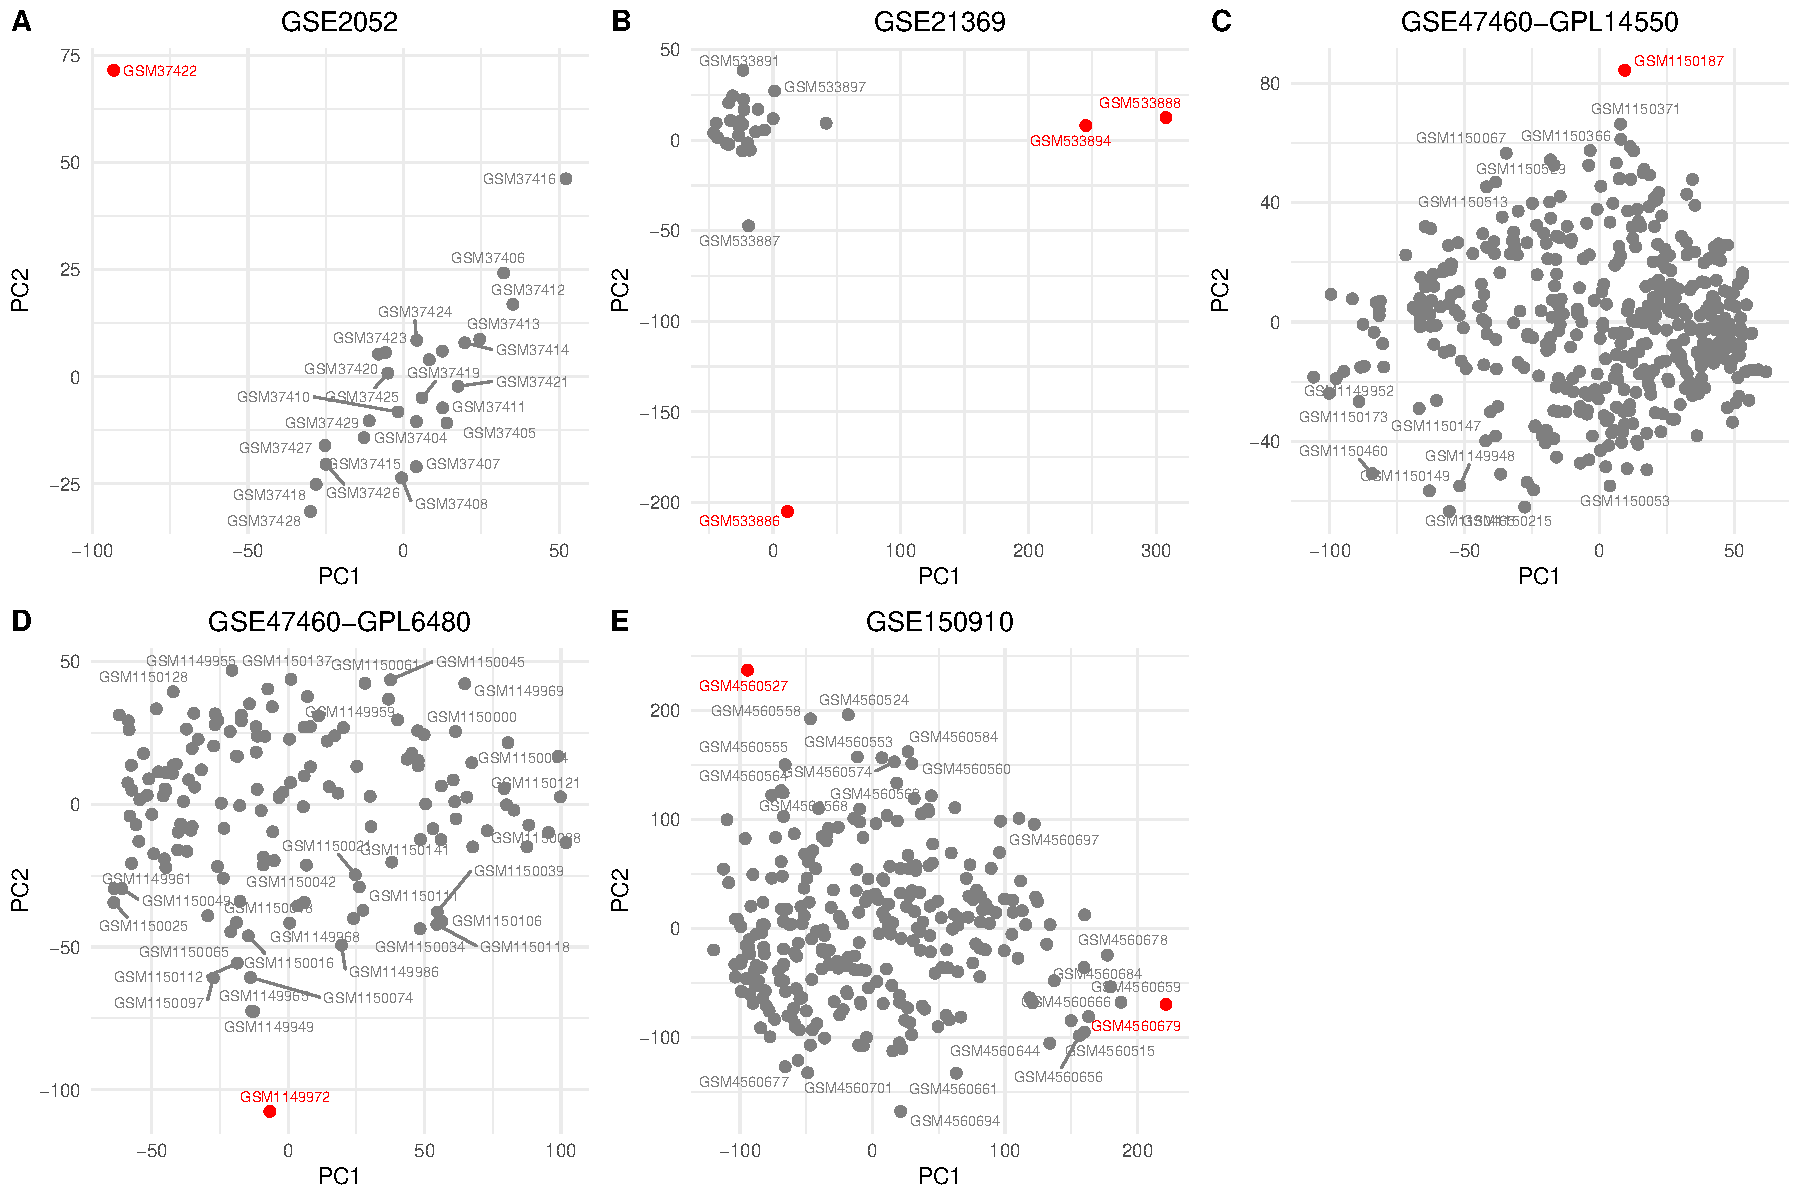
\includegraphics[width=1\linewidth,]{./Figures/FigE1_outliers} \caption[Outlier detection]{\textbf{Sample outlier detection.} Principal component analysis (PCA) of author-normalized expression matrices to identify data outliers (defined as being 3 standard deviations away from the mean of principal component 1 or 2).}\label{fig:outlierPCA}
\end{figure}

\hypertarget{data-integration-and-analysis}{%
\subsection{Data integration and analysis}\label{data-integration-and-analysis}}

The Multivariate INTegrative (MINT) method (`mixOmics' v6.22.0) is based on partial least squares (PLS) regression. In PLS discriminant analysis (PLS-DA), latent components are constructed from linear combinations of the data matrix X variables and Y outcome to maximize covariance, and each variable is assigned a weight coefficient to indicate its importance in defining the component. PLS can also be extended to integrate data across studies (multi-group PLS), by defining global components to project samples from different studies into a common space. The MINT algorithm combines these two approaches and applies a least absolute shrinkage and selection operator (lasso) penalization for variable selection resulting in simultaneous batch correction and classification. MINT classification models are also able to handle missing data via nonlinear iterative partial least squares (NIPALS) modelling {[}\protect\hyperlink{ref-wold_nonlinear_1973}{96}{]}, so they may be applied despite missing probes or reads in the sequencing method of choice.

Datasets were integrated via shared genes and projected into a common latent space via lasso-penalized multi-group PLS (Figure \ref{fig:integration}), which identifies a small subset of variables that can discriminate classes across studies. Tuning of the lasso penalty parameter was performed via leave-one-group-out cross validation, where the optimal model was selected based on the lowest balanced error rate (BER; the average error rate in each class) with a minimum of 50 features to identify biologically important genes (Figure \ref{fig:tuningMINT}). Final model performance was then assessed using the mixOmics `perf' function against the 8 left-out test datasets, and 95\% confidence intervals obtained using the bootstrap method (Table \ref{tab:modelPerf}). Sex-specific models were also generated (Table \ref{tab:sexModel})



\begin{figure}
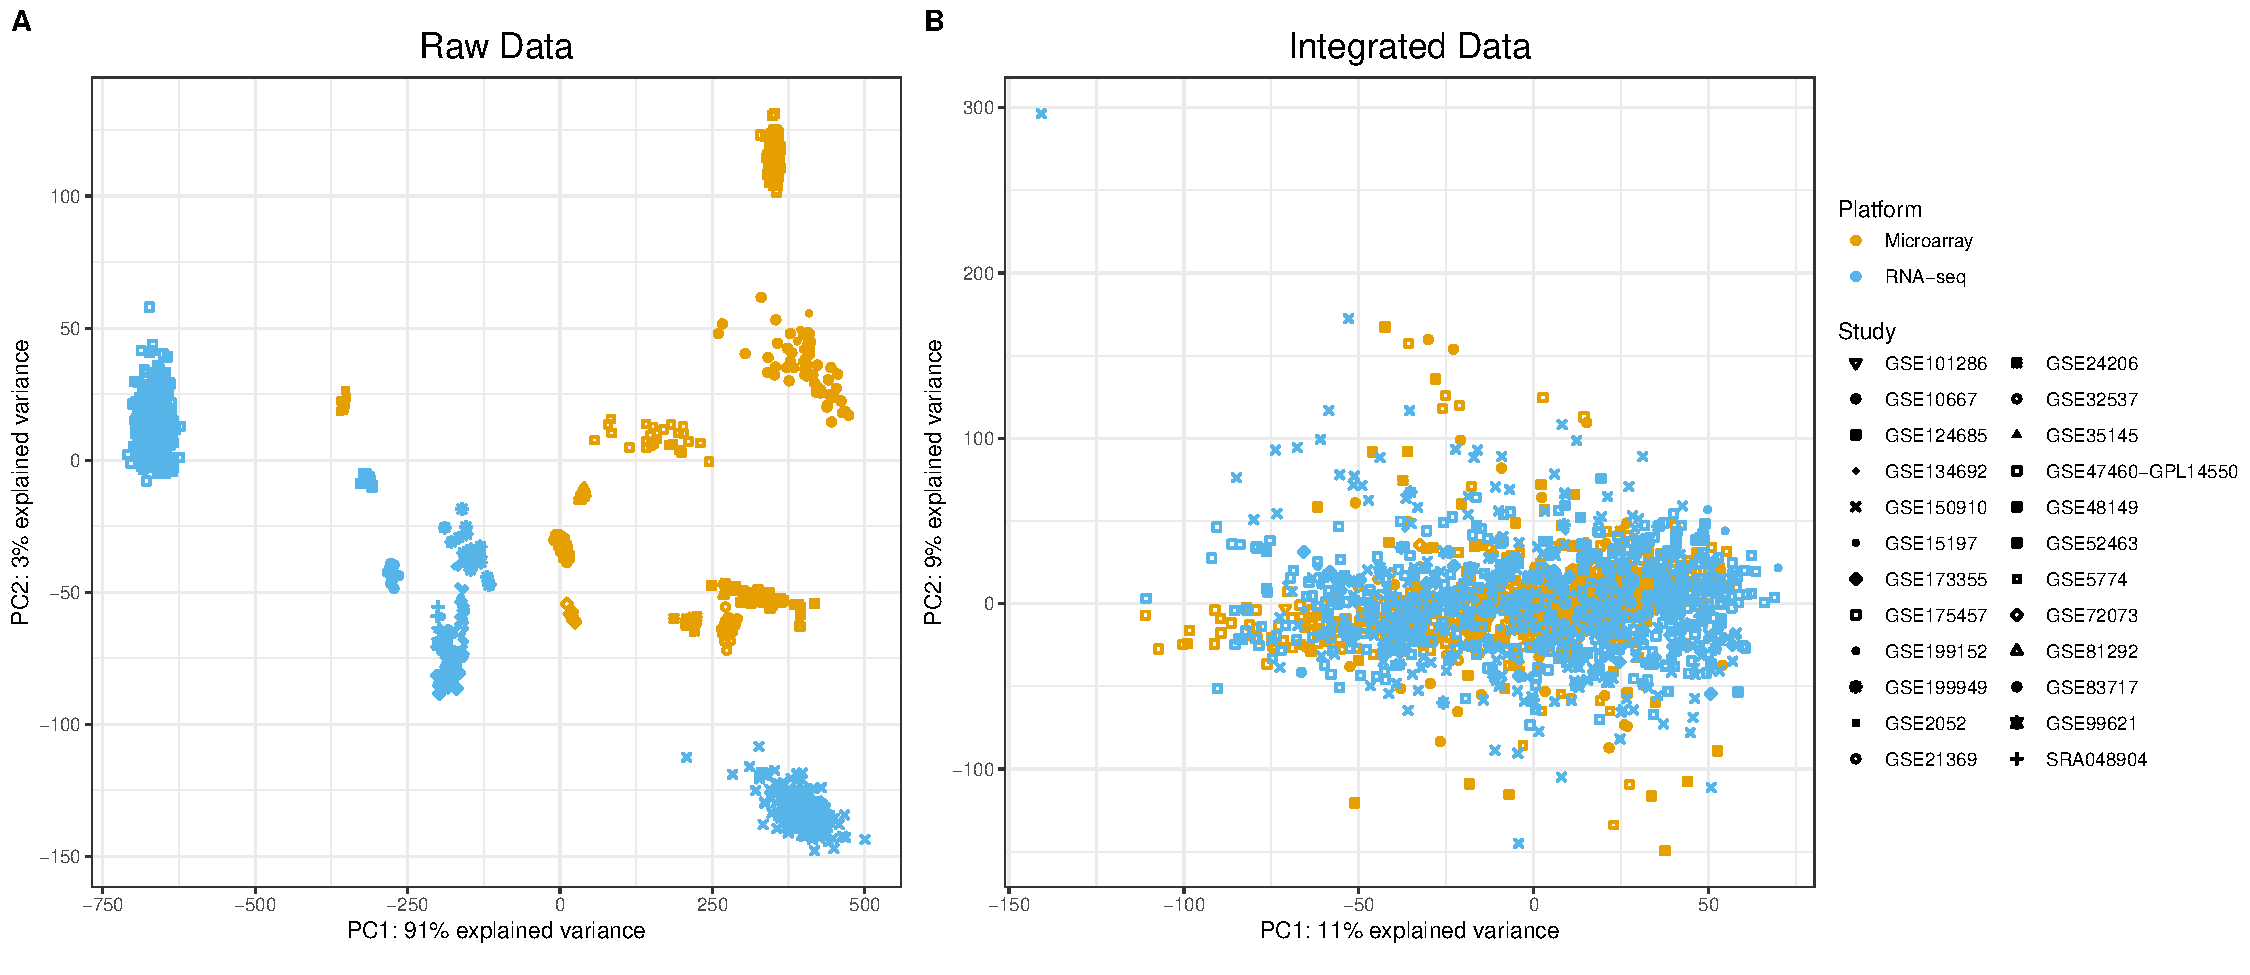
\includegraphics[width=1\linewidth,]{./Figures/Figure2_PCA} \caption[MINT integration]{\textbf{Principal component analysis (PCA) of lung transcriptomics data prior to and after MINT integration.} Author-normalized datasets were subsetted with genes shared in \textgreater80\% of datasets (A) and integrated using MINT. MINT-integrated samples projected into a common latent space via multi-group PCA are shown in (B).}\label{fig:integration}
\end{figure}



\begin{figure}
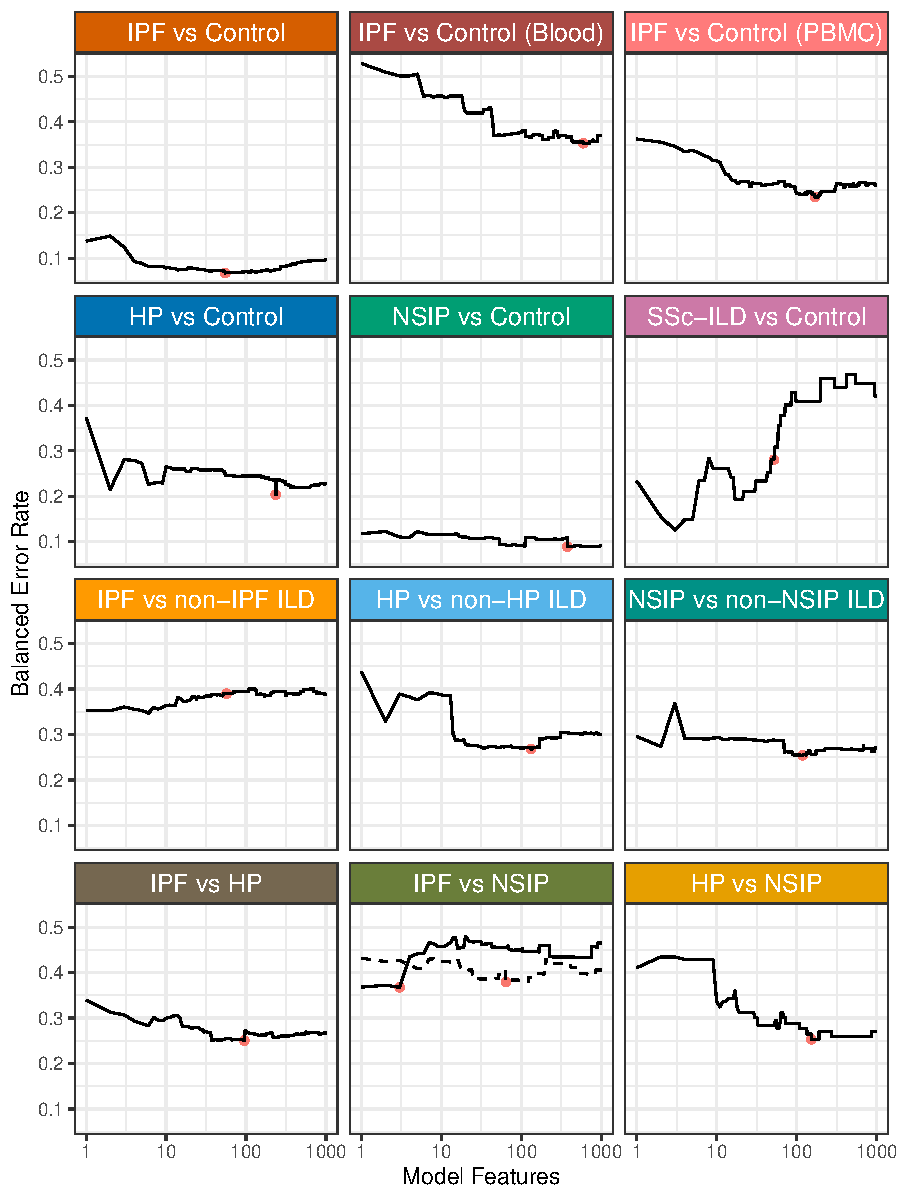
\includegraphics[width=1\linewidth,]{./Figures/FigE2_tuning} \caption[Model tuning]{\textbf{Feature selection for MINT classification models.} Tuning grids to determine the optimal number of features (indicated by red point) for each model based on the lowest balanced error rate. All models were selected based on the lowest BER with a minimum of 50 features. For each model, one PLS component (solid line) was sufficient to separate classes with the exception of IPF vs NSIP, which required a second PLS component (dotted line).}\label{fig:tuningMINT}
\end{figure}

\captionsetup{width=6.5in}



\begin{table}[!h]
\centering\centering
\caption{\label{tab:modelPerf}\textbf{Summary of ILD MINT model performance on indicated test sets.} Area under receiver operating curve (AUC), balanced error rate (BER), sensitivity, and specificity were calculated using the `auroc.mint.splsda' function from mixOmics. 95\% confidence intervals (95\% C.I.) were determined via bootstrapping.}
\centering
\begin{tabu} to \linewidth {>{\raggedright\arraybackslash}p{1.75in}>{\centering\arraybackslash}p{0.5in}>{\centering\arraybackslash}p{0.7in}>{\centering\arraybackslash}p{1.25in}>{\centering\arraybackslash}p{1.25in}}
\toprule
Model & Genes & Test Sets & AUC [95\% C.I.] & BER [95\% C.I.]\\
\midrule
IPF vs Control & 55 & 8 & 0.99 [0.99-1.00] & 0.06 [0.03-0.08]\\
HP vs Control & 235 & 3 & 0.91 [0.84-0.99] & 0.13 [0.05-0.23]\\
NSIP vs Control & 378 & 4 & 0.94 [0.88-0.99] & 0.18 [0.08-0.28]\\
SSc-ILD vs Control & 52 & 1 & 0.98 [0.93-1.00] & 0.11 [0.00-0.25]\\
IPF vs nonIPF & 57 & 6 & 0.71 [0.63-0.79] & 0.35 [0.28-0.43]\\
HP vs nonHP & 132 & 2 & 0.76 [0.63-0.89] & 0.30 [0.18-0.44]\\
NSIP vs nonNSIP & 174 & 4 & 0.60 [0.49-0.72] & 0.46 [0.34-0.58]\\
IPF vs HP & 95 & 3 & 0.76 [0.64-0.87] & 0.28 [0.19-0.39]\\
IPF vs NSIP & 67 & 4 & 0.76 [0.64-0.88] & 0.32 [0.21-0.45]\\
HP vs NSIP & 153 & 2 & 0.74 [0.51-0.96] & 0.37 [0.16-0.60]\\
IPF vs Control (Blood) & 518 & 2* & 0.74 [0.67-0.81] & 0.34 [0.28-0.42]\\
IPF vs Control (PBMC) & 169 & 2** & 0.73 [0.65-0.81] & 0.33 [0.26-0.42]\\
\bottomrule
\multicolumn{5}{l}{\rule{0pt}{1em}* Performance on PBMC datasets}\\
\multicolumn{5}{l}{\rule{0pt}{1em}** Performance on whole blood datasets}\\
\end{tabu}
\end{table}



\begin{table}[!h]
\centering\centering
\caption{\label{tab:sexModel}\textbf{Summary of ILD sex-specific model performance on indicated test sets.} Area under receiver operating curve (AUC), balanced error rate (BER), sensitivity, and specificity were calculated using the `auroc.mint.splsda' function from mixOmics. 95\% confidence intervals (95\% C.I.) were determined via bootstrapping.}
\centering
\begin{tabu} to \linewidth {>{\raggedright}X>{\centering}X>{\centering}X>{\centering}X}
\toprule
Model & Test Datasets & AUC & BER\\
\midrule
IPFmale & Male & 0.98 [0.97-1.00] & 0.08 [0.05-0.13]\\
IPFmale & Female & 0.94 [0.92-0.96] & 0.09 [0.06-0.11]\\
IPFfemale & Female & 0.99 [0.96-1.00] & 0.04 [0.00-0.09]\\
IPFfemale & Male & 0.93 [0.91-0.95] & 0.06 [0.04-0.07]\\
HPmale & Male & 0.96 [0.89-1.00] & 0.11 [0.02-0.20]\\
HPmale & Female & 0.90 [0.84-0.95] & 0.15 [0.10-0.21]\\
HPfemale & Female & 0.88 [0.75-1.00] & 0.20 [0.07-0.35]\\
HPfemale & Male & 0.96 [0.93-0.99] & 0.10 [0.05-0.15]\\
NSIPmale & Male & 0.98 [0.93-1.00] & 0.15 [0.06-0.24]\\
NSIPmale & Female & 0.79 [0.68-0.90] & 0.26 [0.17-0.35]\\
NSIPfemale & Female & 0.88 [0.77-1.00] & 0.15 [0.05-0.27]\\
NSIPfemale & Male & 0.89 [0.78-0.99] & 0.18 [0.08-0.29]\\
\bottomrule
\end{tabu}
\end{table}



\begin{figure}
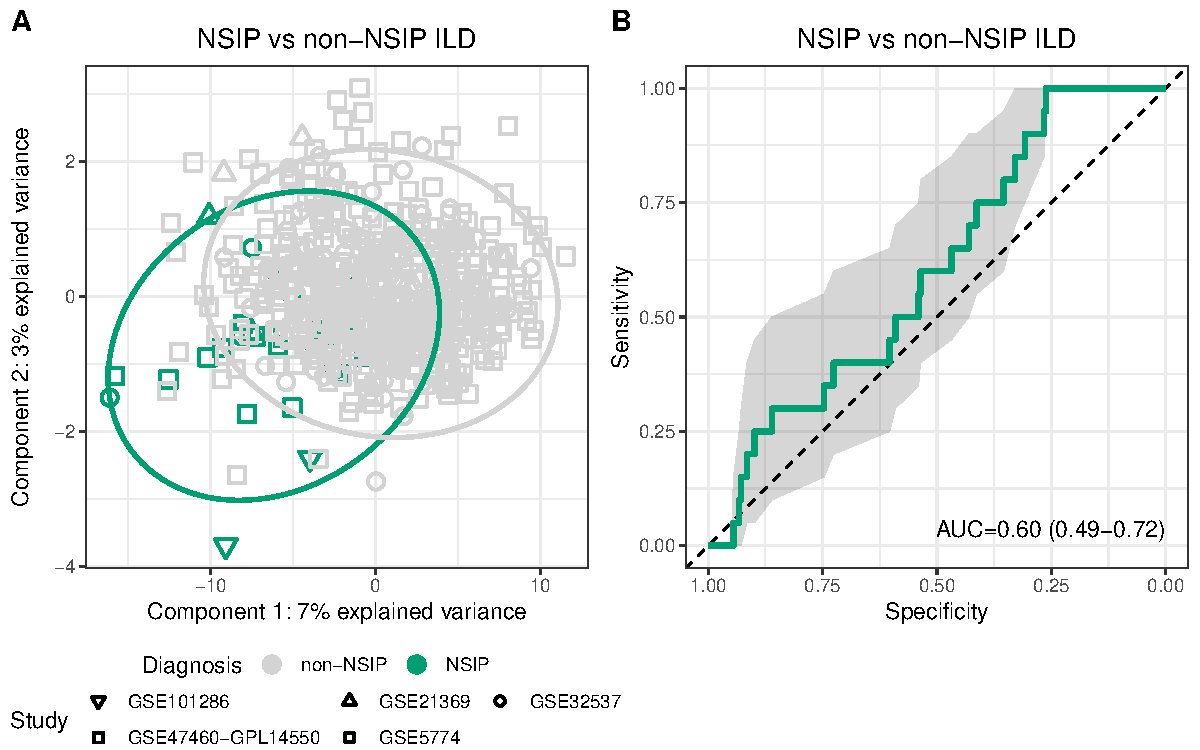
\includegraphics[width=1\linewidth,]{./Figures/FigE5_NSIP} \caption[Model tuning]{\textbf{NSIP-specific classification model.} PLS projection of samples using the NSIP vs non-NSIP ILD model (A) and the AUC performance on held-out test datasets (B).}\label{fig:nsipmodel}
\end{figure}



\begin{figure}
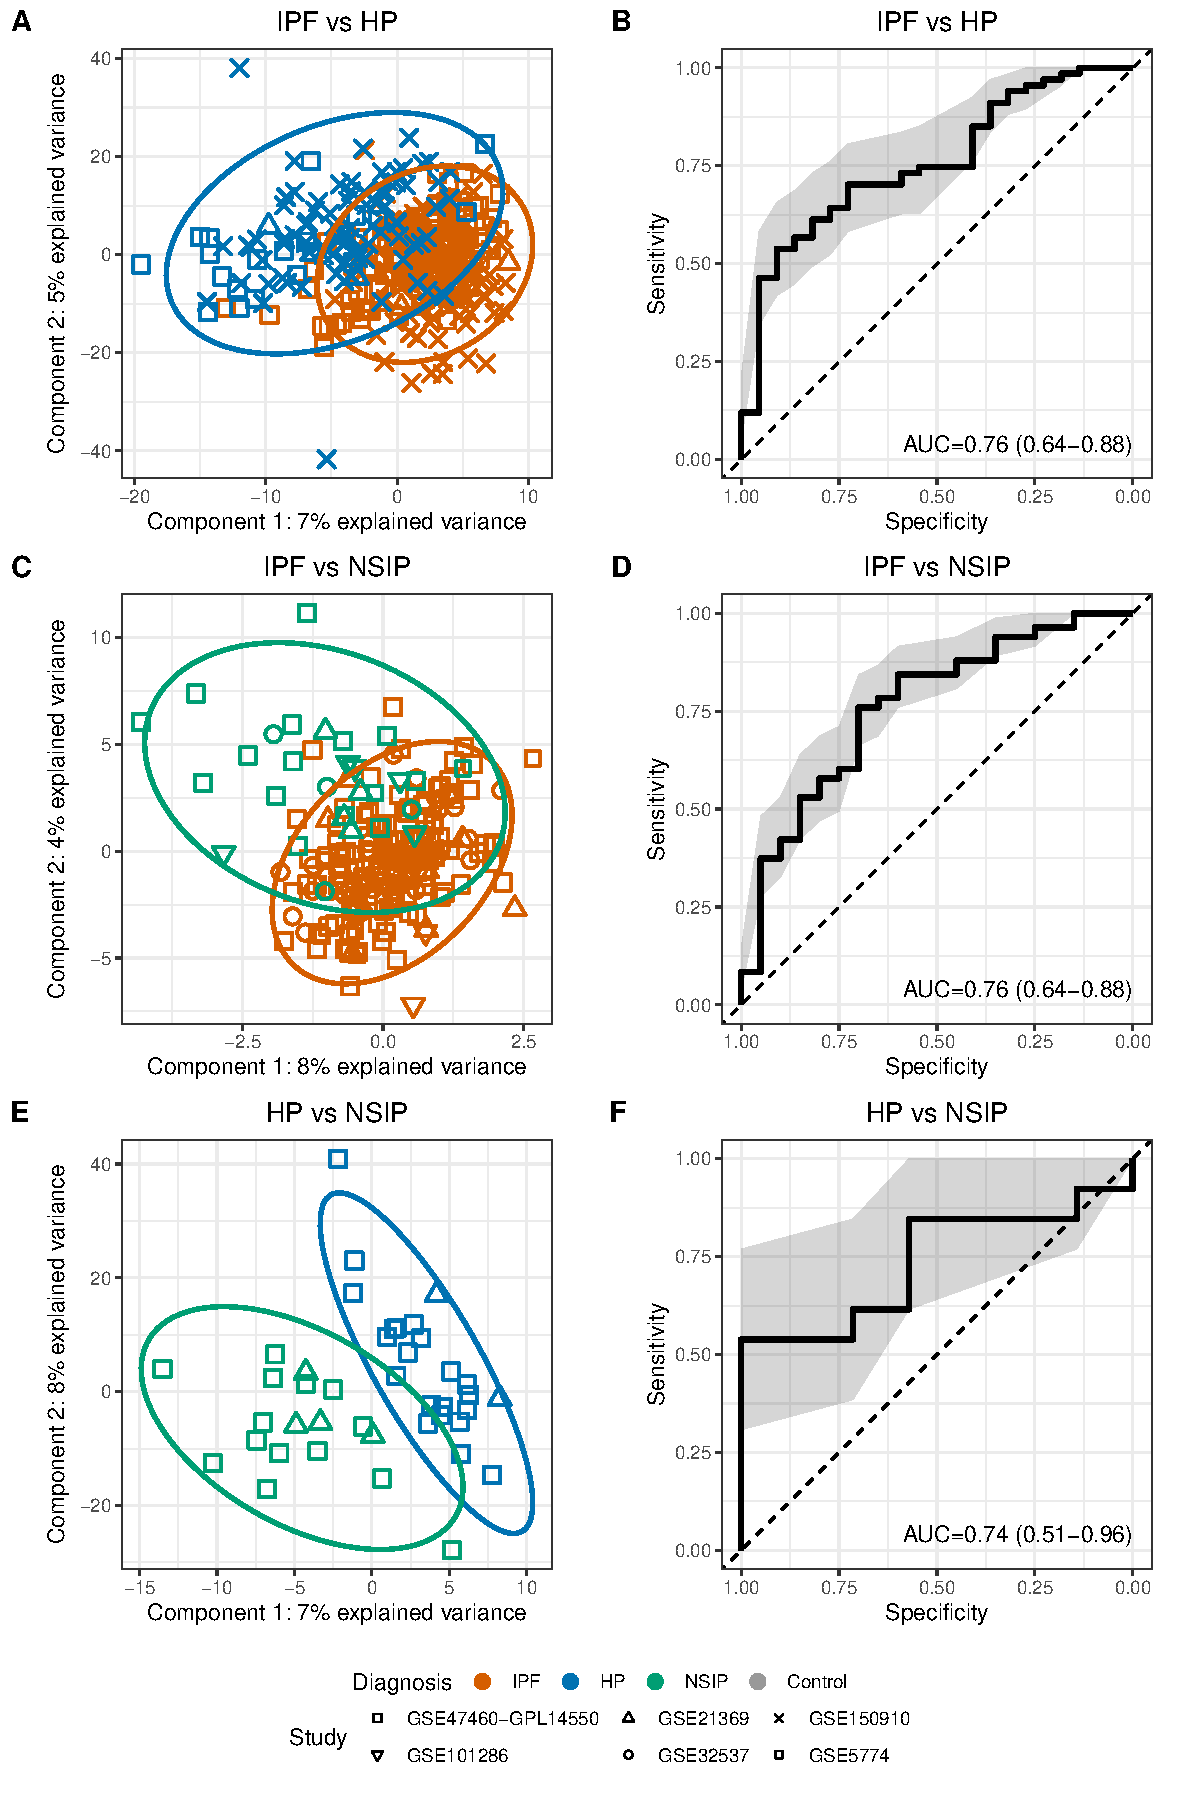
\includegraphics[width=1\linewidth,]{./Figures/FigE6_ILDvsILD} \caption[Individual ILD vs ILD]{\textbf{Classification models differentiating between specific ILD subtypes.} PLS sample projections and held-out test set AUC performance for comparisons between IPF and HP (A, B), IPF and NSIP (C, D), and HP and NSIP (E, F).}\label{fig:ildvsildspecific}
\end{figure}

Pathway analyses were limited for some of our models given their relatively small number of features (e.g.~55 genes for IPF vs Control). To address this, we used the R package `bcp' (version 4.0.3) to determine models with an ``expanded'' number of features. Briefly, data from the tuning grids was analyzed to identify changepoints (i.e.~points at which the BER was likely to change). We selected the most amount of features at which the BER remained stable before increasing, as this would provide us with a high number of features without sacrificing model performance. To ensure that the expanded models recapitulated the performance of the original model, we applied them to the test sets to confirm their ability to discriminate between classes (data not shown).
Gene lists from expanded models were then analyzed via overrepresentation analysis using the `cashoes/sear' package (\url{https://github.com/cashoes/sear}) (Table E8).
Custom cell pathway annotations were used for Table E9 based upon single-cell RNA-seq data from (16--19).

\hypertarget{biclustering-1}{%
\subsection{Biclustering}\label{biclustering-1}}

In MoSBi (v1.4.0), biclusters are identified via biclustering algorithms (bimax, fabia, isa2, plaid, QUBIC) {[}\protect\hyperlink{ref-rose_mosbi_2022}{52}{]}. UnPaSt is an \href{https://github.com/ozolotareva/UnPaSt}{unconstrained version} of the method published in {[}\protect\hyperlink{ref-zolotareva_identification_2021}{53}{]}. Ensemble biclusters from the identified biclusters are determined through Louvain community aggregation, while a similar procedure was performed for UnPaSt biclusters using weighted gene co-expression network analysis.

Biclusters were filtered to select for those enriched in specific lung disease groups (control, IPF, HP, NSIP, COPD). We also included CTD-ILD (including unspecified CTD-ILD subtypes, RA-ILD, SSc-ILD) and other ILD (acute interstitial pneumonia, COP, CPFE, DIP, IPF-acute exacerbation, RB-ILD, unknown fibrosis) samples in our biclustering analysis to increase the number of ILD samples; however, these were not used in filtering for biclusters enriched in specific disease groups. Final biclusters were named sequentially with an M- prefix if identified from MoSBi or a U- prefix if identified by UnPaSt. Genes in each bicluster can be found in INSERT LINK.

\hypertarget{appendix-b---supplementary-information-for-chapter-three}{%
\subsection{Appendix B - Supplementary information for Chapter Three}\label{appendix-b---supplementary-information-for-chapter-three}}

\renewcommand{\thefigure}{A3.\arabic{figure}}
\setcounter{figure}{0}
\renewcommand{\thetable}{A3.\arabic{table}}
\setcounter{table}{0}
\renewcommand{\theequation}{A3.\arabic{equation}}
\setcounter{equation}{0}

\hypertarget{appendix-c---supplementary-information-for-chapter-four}{%
\subsection{Appendix C - Supplementary information for Chapter Four}\label{appendix-c---supplementary-information-for-chapter-four}}

\renewcommand{\thefigure}{A4.\arabic{figure}}
\setcounter{figure}{0}
\renewcommand{\thetable}{A4.\arabic{table}}
\setcounter{table}{0}
\renewcommand{\theequation}{A4.\arabic{equation}}
\setcounter{equation}{0}

\end{document}
